\documentclass{article}
\usepackage[english]{babel}
\usepackage[utf8]{inputenc}
\usepackage{johd}
\usepackage{array}
\usepackage{setspace}
\usepackage{graphicx}
\usepackage{multirow}
\usepackage{subcaption}
\usepackage{hyperref}
\usepackage{titling} 
\onehalfspacing
\setlength{\parskip}{1em} 
\setlength{\parindent}{0pt}
\usepackage[backend=biber,style=numeric,sorting=none]{biblatex}  
\addbibresource{thesis.bib} 


\begin{document}

% Title Page
\begin{titlepage}
    \centering
    {\LARGE \textbf{Optimizing Defensive Positioning for Columbia University Baseball Based on Batter-Pitcher Handedness}} \\[1.5cm] 
    
    \vspace{5cm}
    
    {\large A Thesis submitted to the Faculty of the Department of Computer Science at Columbia University in partial fulfillment of the requirements for the degree of Bachelor of Arts in Computer Science} \\[2cm]

    \vspace{5cm} 
    
    {\large By: Lillian M. Bradley, lmb2313} \\[0.5cm]
    
    
    \vfill 

    {\large New York, New York} \\[0.5cm]
    {\large May 10, 2025}
\end{titlepage}


\pagenumbering{gobble}
\begin{center}
    {\textbf{Optimizing Defensive Positioning for Columbia University Baseball Based on Batter-Pitcher Handednes}} \\[1cm]
    {Lillian M. Bradley} \\[0.5cm]
    {Thesis Advisor: Dr. Andrew J. Blumberg} \\[2cm]
\end{center}
\begin{abstract} 
Defensive positioning is a crucial aspect of baseball, influencing the probability of converting balls in play into outs. While traditional positioning strategies rely on player intuition and experience, data-driven approaches can optimize defensive alignment based on batter-pitcher match-ups. This project aims to develop a predictive model to optimize defensive positioning for Columbia University Baseball, leveraging TrackMan data and advanced machine learning techniques. TrackMan data from the 2022-2024 seasons was used to train an XGBoost model, predicting the optimal defensive positions for each player based on batter-pitcher handedness. Key features included batter and pitcher handedness, player position (X, Z coordinates), and infield shifting. The model achieved an accuracy of $75.50\%$, accurately predicting the optimal defensive positioning for each player. Significant positional shifts were observed for players based on batter-pitcher match-ups, especially for middle infielders. The optimized defensive positioning model provides actionable insights for Columbia Baseball and can be adapted for other NCAA teams, enabling them to adjust fielding positions based on real-time batter-pitcher match-ups. Future work could include incorporating additional features, such as weather data, hit location data, and player-specific attributes, to further improve the model's accuracy.
\end{abstract}

\newpage
\pagenumbering{gobble}
\begin{center}
    \textbf{\large Acknowledgments}
\end{center}
 This research was greatly supported by my thesis advisor, Dr. Andrew J. Blumberg, whose guidance was instrumental throughout this project and my time at Columbia, and by my Applied Machine Learning professor, Dr. Wayne Tai Lee, whose expertise also contributed to the success of this work. I would also like to thank Columbia University Baseball and the Columbia University SabrLions for granting me access to their data for this project. I am deeply grateful to my father, Brendan Bradley, for his unwavering support and guidance throughout my life, always encouraging me to follow my passions and challenge myself, and for passing down his love for mathematics and technology to me. Without him, none of this would have been possible.


\newpage
\pagenumbering{gobble}
\tableofcontents

\newpage
\pagenumbering{arabic}
\section{Introduction}
\subsection{Basics of Baseball}
For this thesis, I will be looking at NCAA Division I \cite{ncaa2023baseballrules} and Major League Baseball's  \cite{mlb2025officialrules} baseball rules and regulations.

Baseball is played on a diamond-shaped field with four bases: home plate, first base, second base, and third base. The area inside the base path is called the infield, while the area beyond it is the outfield. 

A standard baseball game lasts nine innings, though this can vary at different levels and with specific game circumstances. Each inning is split into two halves:

\begin{itemize}
    \item In the \textbf{top} of an inning, the away team bats while the home team plays defense
    \item In the \textbf{bottom} of an inning, the teams switch roles 
\end{itemize}

\subsubsection{Defensive Positions} 
At any given time, there are nine defensive players on the field, \cite{wikipedia2023baseballpositions}:
\begin{itemize}
    \item \textbf{Pitcher (P)(1):} Stands on the pitcher's mound and throws the ball to the batter
    \item \textbf{Catcher (C)(2):} Positioned behind home plate and responsible for catching the ball from the pitcher
\end{itemize}

\textbf{Infield:}
\begin{itemize}
    \item \textbf{First Baseman (1B)(3):} Covers first base
    \item \textbf{Second Baseman (2B)(4):} Positioned between first and second base
    \item \item \textbf{Third Baseman (3B)(5):} Covers third base
    \item \textbf{Shortstop (SS)(6):} Positioned between second and third base
\end{itemize}

\textbf{Outfield:}
\begin{itemize}
    \item \textbf{Left Fielder (LF)(7):} Covers the left side of the outfield
    \item \textbf{Center Fielder (CF)(8):} Positioned in the middle of the outfield; covers a large amount of the outfield
    \item \textbf{Right Fielder (RF)(9):} Covers the right side of the outfield
\end{itemize}

\begin{figure}[h]
    \centering        
    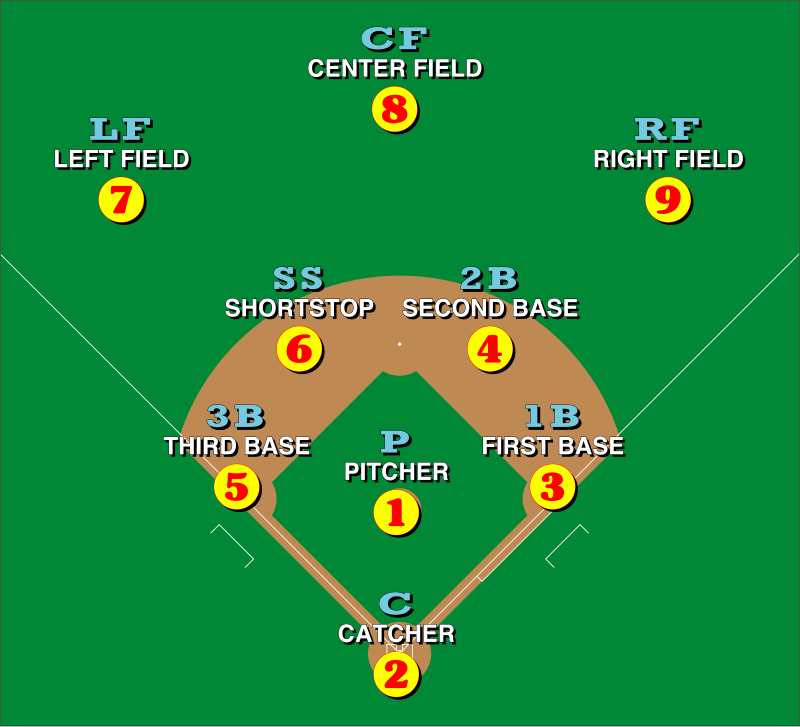
\includegraphics[height=10cm]{images/Baseball_positions.svg.png}
    \caption{Baseball Field with Defensive Positions Labeled}
    \cite{wikipedia2023baseballpositions}
\end{figure}
\vspace{3cm}
\newpage

\subsubsection{Batting and Scoring} 
Each defensive player except the pitcher bats as a part of the team's offense. In MLB and at the NCAA Division I level, there is a "designated hitter (DH)" who will be the ninth player to hit for a team; the pitcher can be the designated hitter but does not have to be. 

The coaching staff decides before each game which players will play which positions and the order that they will hit in. This order remains constant throughout the game. The game begins with the away team's lead-off hitter coming up to bat. 

\subsubsection{Balls, Strikes, and Outs} 
Each at bat begins with an 0-0 count. 

\begin{itemize}
    \item If a pitch misses the strike zone \cite{mlb2023strikezone} - a predetermined box spanning from the batter's armpits to  the bottom of his knees - and the batter does not swing, it is ruled a \textit{ball}
    \item If a batter receives four balls during an at bat, they are awarded first base; this is known as a \textit{walk}

    \item If a batter swings and misses or the ball crosses the plate in the strike zone, the pitch is ruled a \textit{strike}
    \item If a batter accumulates three strikes, then they are \textit{out}

    \item A ball that is hit into foul territory - the area to the right of first base and to the left of third defined by distinct white lines on the field - is:

    \begin{itemize}
        \item counted as a strike if the batter has fewer than two strikes
        \item never counted as the third strike
        \item an out, if it is caught by a defensive player
    \end{itemize}
\end{itemize}

Any hit, including a foul ball, is ruled as an out when it is caught by a defensive player. Batters will come up to hit in their predetermined order and after three outs, the teams switch roles. 

\subsubsection{Game Duration and Special Rules}
At the Major League Level, games are played for a minimum of nine innings. If the home team leads after the top of the ninth, the game is over immediately and they have won. If the game is tied after nine innings, it continues into extra innings until one team has a higher score after a full inning. \cite{mlb2025officialrules}

At NCAA Division I level, the same rules apply, but a mercy rule can be used. Before the game, both team's head coaches can agree to a rule that if one team leads by ten or more runs after seven innings, the game ends early. \cite{ncaa2023baseballrules}



\subsection{Background on Baseball Defensive Positioning}
\subsubsection{General Principles of Defensive Alignment}
In a baseball game there are nine defensive players on the field: the pitcher, catcher, first baseman, second baseman, third baseman, shortstop, left fielder, center fielder, right fielder. I will be examining the locations of seven of these positions, the first baseman, second baseman, third baseman, shortstop, left fielder, center fielder, right fielder. The first, second, third baseman, and shortstop make up the infield positions. Typically, the first and second baseman will be on the right side of second base, and the shortstop and third baseman on the left side. There is a rule called the shift, that I will explain in the next section (\ref{sec:defensive_shifts}), where this changes a bit. The left fielder, center fielder, and right fielder make up the outfield, the area behind the base-paths, and each is loosely positioned to match their name. Below is an image of a baseball field with the defensive positions labeled. 


\subsubsection{Infield Alignments and The Defensive Shift} \label{sec:defensive_shifts}
Major League Baseball groups all infield defensive alignment into one of the following four categories \cite{mlb2023shifts}:

\begin{itemize}
    \item \textbf{Standard:} All four infielders are positioned in a basic/typical/traditional spot on the field
    \item \textbf{Shift:} Three or more infielders on the same side of second base
    \item \textbf{Shaded:} At least one fielder is positioned outside the area of the field they're typically responsible for. (Example: The SS is "shaded" when playing up the middle against a LHB or toward the 3B zone against a RHB)
    \item \textbf{Strategic:} Any other tactical alignment. (Examples: an infielder playing in or holding the line, an outfield rover, a fifth infielder, etc.)
\end{itemize}



\newpage
\begin{figure}[h] 
    \centering  
    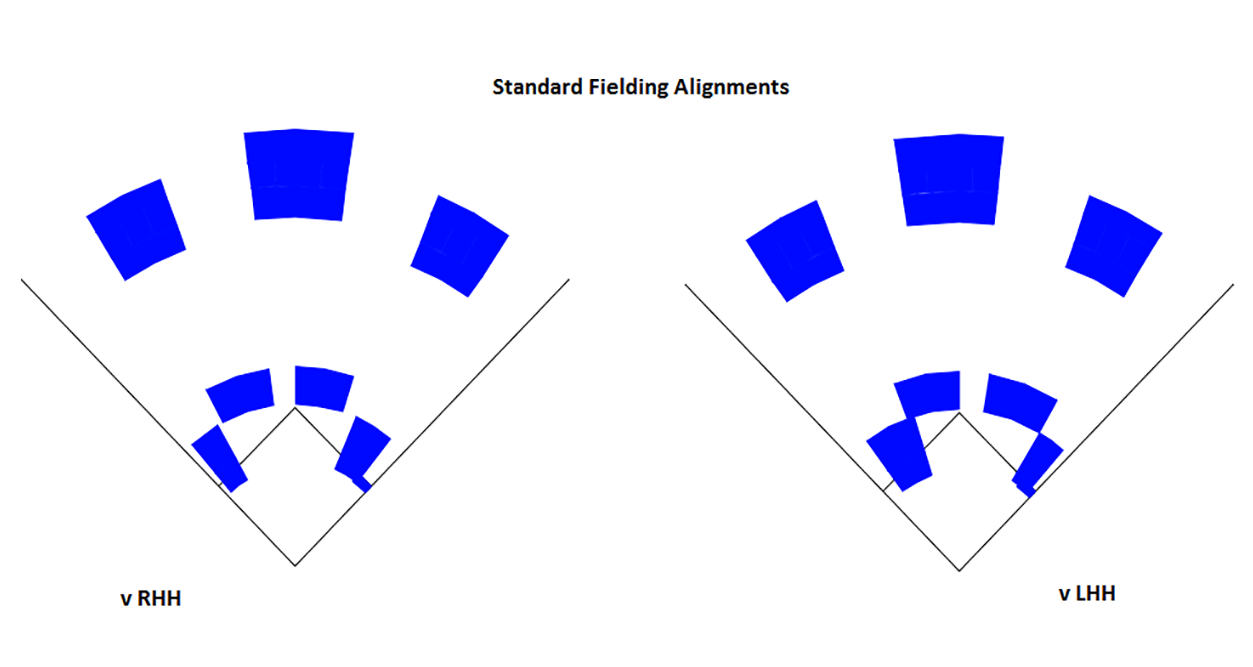
\includegraphics[height=9cm]{images/standard.png}
    \caption{Standard Infield Positioning Against Right Handed Hitters and Left Handed Hitters}
    \cite{mlb2023shifts}
\end{figure}
Standard alignment is the traditional positioning, essentially the default. It varies slightly depending on the batters hand. 


\newpage


\vspace{1.5cm}
\begin{figure}[h]
    \centering        
    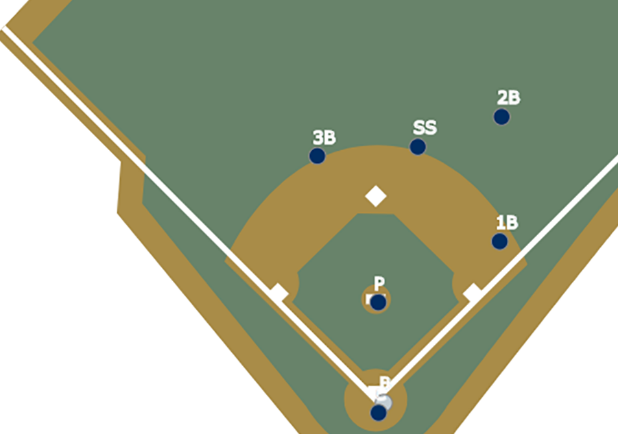
\includegraphics[height=8cm]{images/shift.png}
    \caption{Shifted Infield Positioning}
    \cite{mlb2023shifts}
\end{figure}
\vspace{1.5cm}

The shift was banned by MLB prior to starting the 2023 season. At the major and minor league levels, teams must have all four infielders within the boundary of the infield while the pitcher is on the rubber, infielders are not allowed to switch sides, and two infielders must be on each side of second base at the start of each pitch. \cite{mlb2023shiftlimits}

The shift is still legal at the NCAA level and is often utilized in defensive positioning. It most often occurs when a lefty is at bat due which I will get into in section \ref{sec:platoon}. 


\newpage
\vspace{1.5cm}
\begin{figure}[h]
    \centering        
    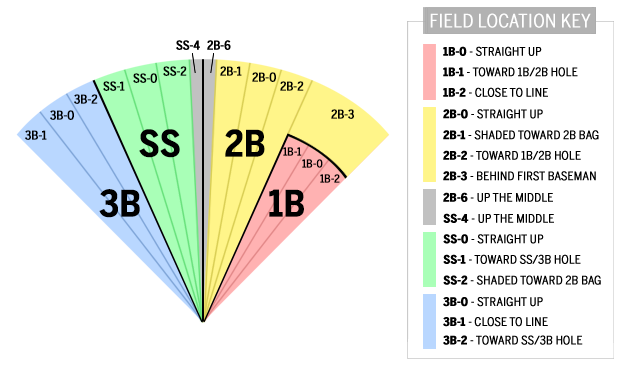
\includegraphics[height=8cm]{images/shaded.png}
    \caption{Shaded Infield Positioning}
    \cite{mlb2023shifts}
\end{figure}
\vspace{1.5cm}
Shaded alignment is essentially the middle ground between the shift and standard. \cite{mlb2023shifts} An infielder is considered to be "shaded" when he is outside of his typical "slice" of the field for his position. This typically means that he has moved to the left or right of his usual positioning. 


\newpage

\vspace{1.5cm}
\begin{figure}[h]
    \centering        
    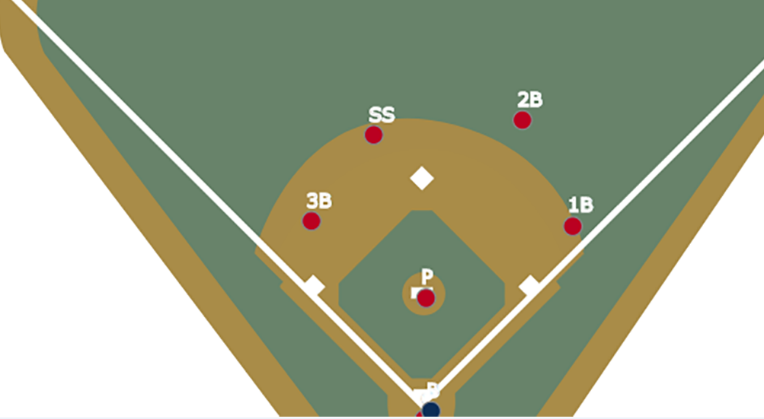
\includegraphics[height=8cm]{images/strategic.png}
    \caption{Strategic Infield Positioning}
    \cite{mlb2023shifts}
\end{figure}
\vspace{1.5cm}
Strategic defensive alignment is an umbrella term for irregular and non-shifted defensive alignment; it can apply to all defensive players not just the infield. Some examples of strategic defensive alignment include bringing the infield in if a bunt is suspected, meaning that the infield positions are closer to home plate, having an outfielder come in to be the "fifth infielder", and as shown below having the second baseman act as a rover. \cite{mlb2023shifts}


\subsubsection{Outfield Alignments}
The outfield's positioning takes into account external factors as well such as wind speed, weather, time of day, and ballpark dimensions. \cite{mlb2023windimpact}\cite{mlbsavant2023catchprobability} Similar to infield positioning grouping, MLB's Statcast groups outfield positioning into one of four of the following categories, \cite{mlb2023shifts}:  

\begin{itemize}
    \item \textbf{Standard:} All three outfielders are positioned in a basic/typical/traditional spot on the field
    \item \textbf{3 Outfielders to one Side of Second Base:} All three outfielders are positioned on the same side of second base
    \item \textbf{4th Outfielder:} A member of the infield, most often the third baseman, moves out into the outfield. This is not allowed in MLB as of 2023, as part of the shift ban. \cite{mlb2023shiftlimits} 
    \item \textbf{Strategic:} Any other tactical alignment that does not fall into a category. This is quite rare at this point in baseball. 
    \caption{Different Outfield Positioning Alignments}
\end{itemize}

\begin{center}
\begin{tabular}{cc}  
    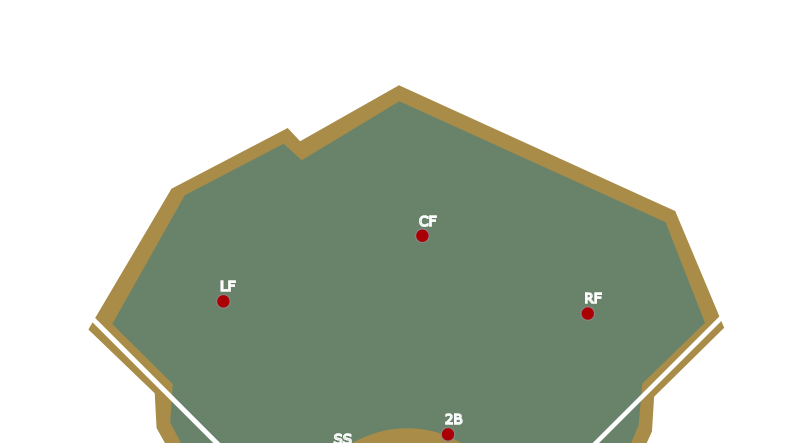
\includegraphics[width=0.5\textwidth]{images/standardOut.png} & 
    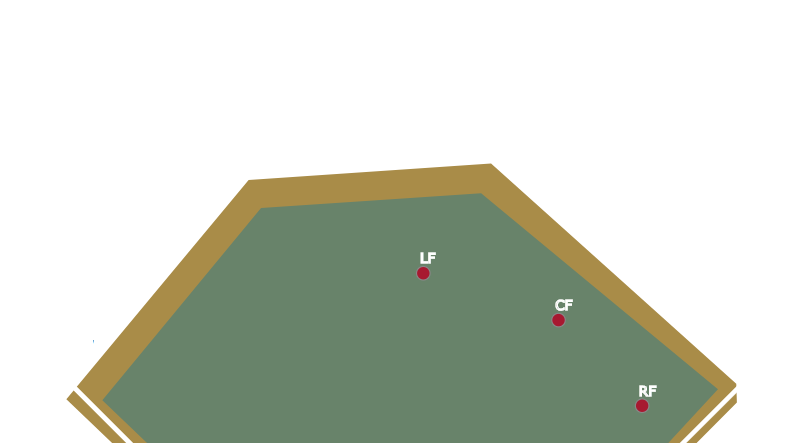
\includegraphics[width=0.5\textwidth]{images/3OF2B.png} \\
    Standard Outfield Positioning & 2 Outfielders on One Side of 2nd Base \\
    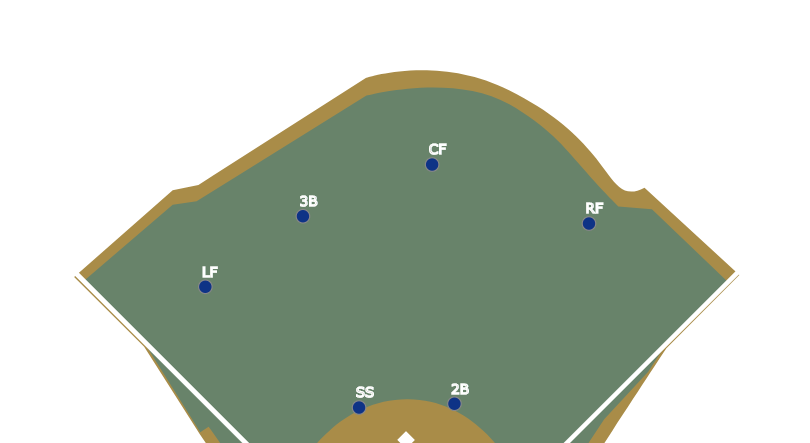
\includegraphics[width=0.5\textwidth]{images/4OF.png} & 
    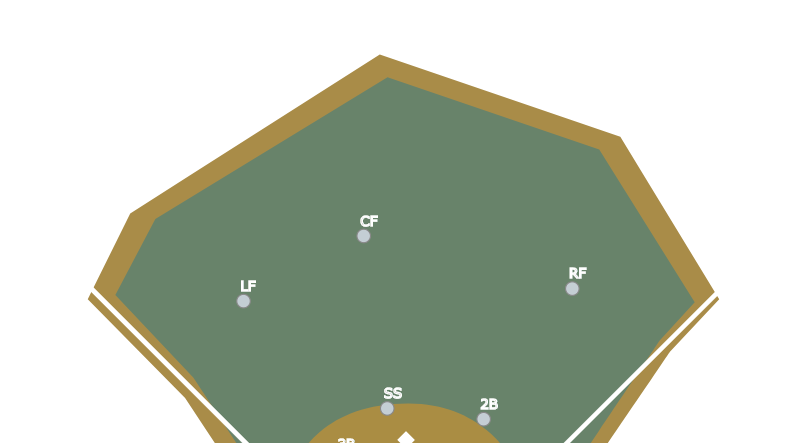
\includegraphics[width=0.5\textwidth]{images/strategicOut.png} \\
    4 Outfielders & Strategic Positioning \\
    \cite{mlb2023shifts}
\end{tabular}
\end{center}
\vspace{1.5cm}

\subsection{Handedness in Baseball}
\subsubsection{How Handedness Affects Batted Ball Direction}
Different players tend to favor hitting to different areas of the field. \cite{mlb2023left-handedpitching,} The basic reasons behind these most common locations is pitcher and batter hand. Hitters are known to pull the ball opposite from their hitting hand - right-handed batters will often pull the ball to their left (right field) while left-handed batters tend to pull to their right (left field). This is due to the natural motion of the swing of a bat. 

There are some players that specialize in opposite field hitting. \cite{ignitebaseball2023pullswing} This is when a batter hits the ball to their "weak side"; for right-handed batters this is right field and for left-handed batters this is left field. Opposite field hitting requires a different plate approach and swing timing. It is usually used when runners are in scoring position (2nd or 3rd base) in the hopes of advancing them.

The natural differences between left-handed and right-handed hitters is shown in the hitting heatmaps below for two of the best hitters in MLB - Shohei Ohtani \cite{mlbsavant2023ohtani}, the left-handed designated hitter for the Los Angeles Dodgers and Mookie Betts \cite{mlbsavant2023betts}, a right-handed hitting utility player for the Los Angeles Dodgers.

\begin{figure}[h]
    \centering
    \begin{tabular}{cc}  
        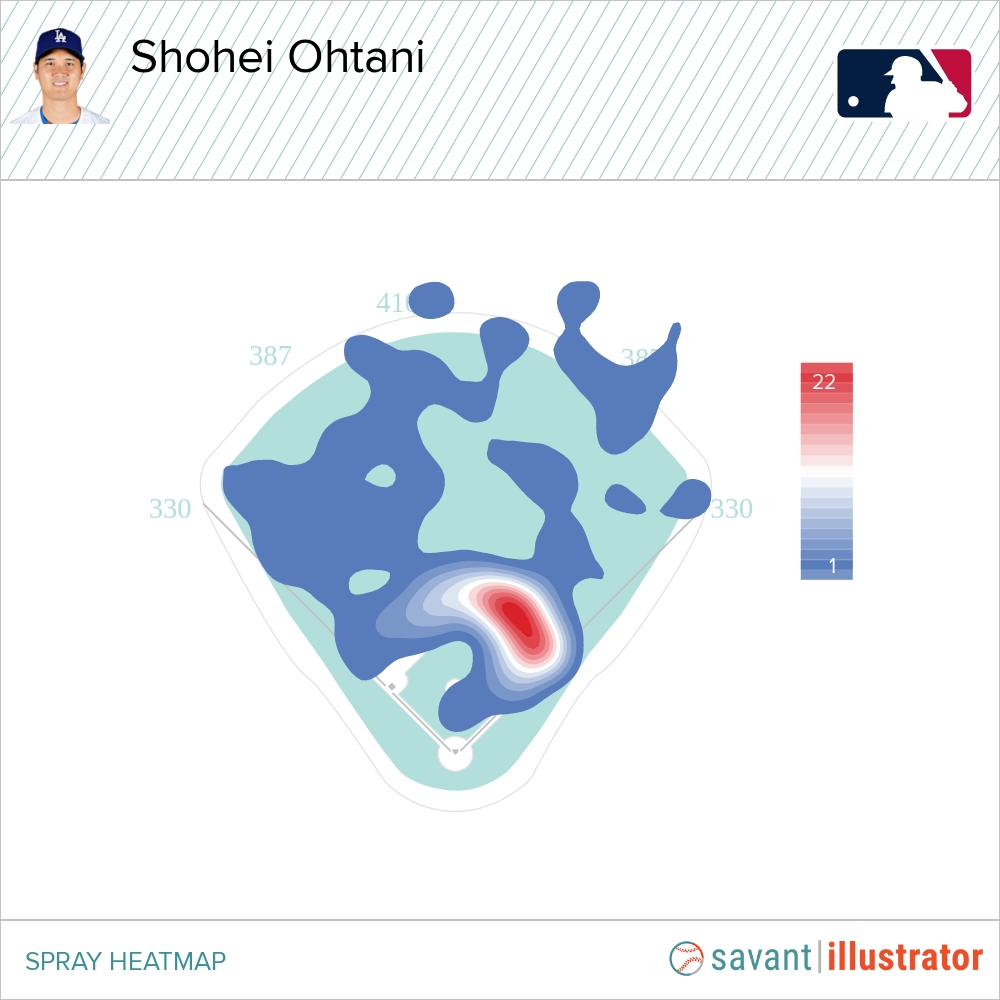
\includegraphics[width=0.5\textwidth]{images/OhtaniHeat.jpg} & 
        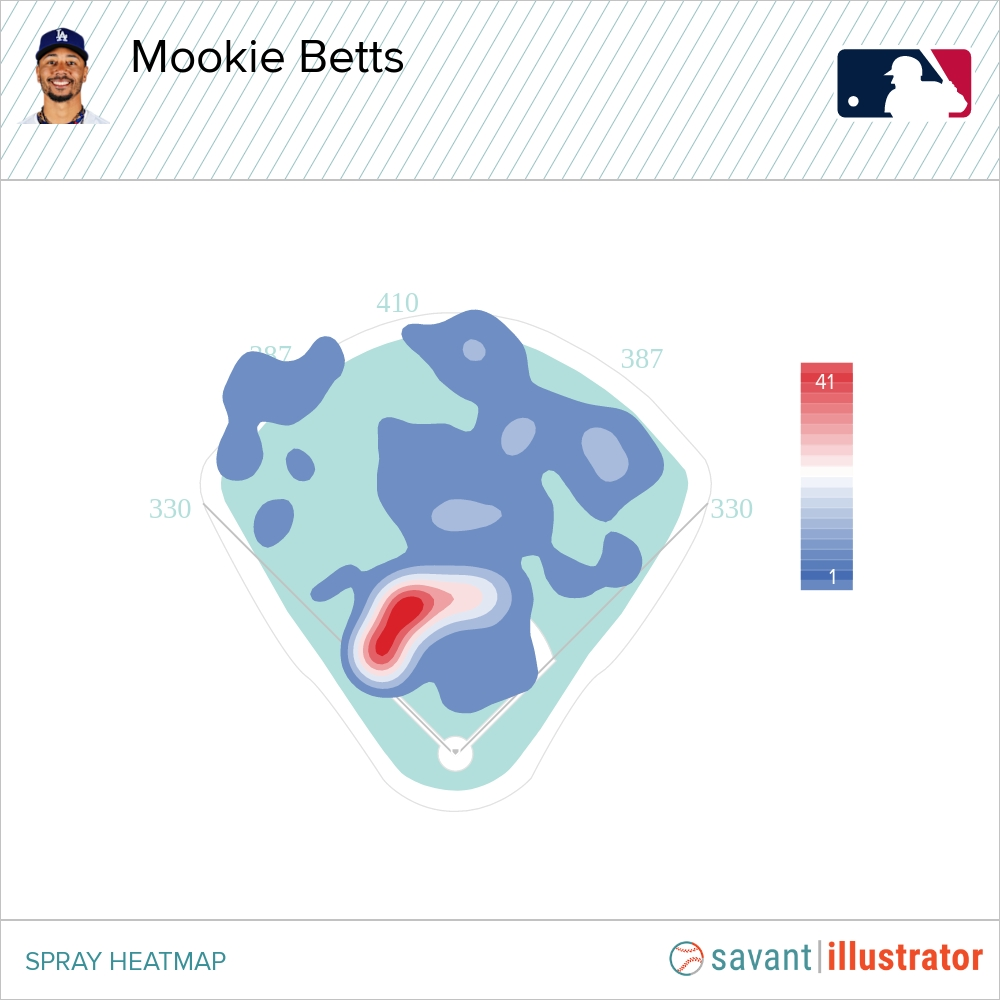
\includegraphics[width=0.5\textwidth]{images/BettsHeat.jpg} \\
        Shohei Ohtani - LHB \cite{mlbsavant2023ohtani} & Mookie Betts - RHB \cite{mlbsavant2023betts}
    \end{tabular}
    \caption{Batted Ball Distribution by Handedness for Two of MLB's Best Hitters – 2024 Season}
    \label{fig:heatmaps}
\end{figure}
\vspace{1.5cm}

\newpage
 



\subsubsection{Platoon Advantage} \label{sec:platoon}
Hitters often have an easier time hitting against opposite-handed pitchers. This is due to the angle of the pitches and the movement of breaking balls - pitches that do not travel straight while approaching the batter. Some breaking balls such as curveballs and sliders will typically curve away from the pitcher's throwing side; a right-handed pitcher's curveball curves away from a right-handed batter but towards a left-handed batter so it is more difficult for the right-handed batter to hit it. A batter's ability to perform better against a pitcher of the opposite hand is known as the "Platoon Advantage" in baseball. 

This advantage is greater for lefties as left-handed hitters do worse against left-handed pitchers than right-handed batters do against right-handed pitchers; this is due to the difference in number of left-handed and right-handed players across baseball. Approximately 10\% of the world's population is left-handed, while this percent is higher in Major League Baseball, the minority still holds true in the baseball world with around 25\% of MLB player's being left-handed. This means that both left-handed pitchers and hitters are less common than right-handed pitchers and hitters. Players will have faced significantly less lefties on both sides of the plate throughput their baseball career, giving them much more experience against righties. \cite{mlb2023left-handedpitching} \cite{appliedvision2023}

It is also worth noting that the left-handed batter's box is physically closer to first base than the right-handed batter's box. A left-handed batter's momentum is also pushing them to first as their body turns towards first base naturally when they swing.

Some teams will platoon certain positions by having two players for it - one left-handed and the other right-handed so they can deploy the player that will hit better based on the handedness of the pitcher they will be facing. It is also common for a team to pinch hit a batter of the opposite hand when a relief pitcher is brought in. 

\vspace{1.5cm}
\begin{figure}[h]
    \centering        
    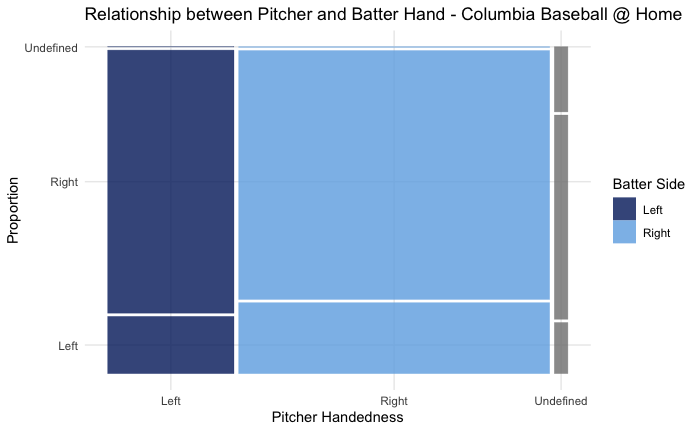
\includegraphics[height=10cm]{images/columbia_handedness.png}
    \caption{Breakdown of match-ups by handedness when Columbia Baseball is pitching at home over the 2022, 2023, and 2024 seasons}
    \cite{columbialions2022baseball}\cite{columbialions2023baseball}\cite{columbialions2024baseball}
\end{figure}
\vspace{1.5cm}


\newpage
\subsection{Problem}
\subsubsection{Why Defensive Optimization is Crucial}
Due to the pull tendencies of batter's and the handedness match-ups, the defensive player's on the field will often adjust their positioning accordingly. Team's will shift and move strategically based on a hitter's tendencies. Adjusting the positioning of player's can minimize runs scored by the opposing team and maximize outs by having players placed in the ideal positions to catch or get to the ball in the current situation. \cite{yanksgoyard2022galloargument} \cite{mlbsavant2023gallobatterpositioning} \cite{fangraphs2023gallo} \cite{mlbsavant2023gallo} \cite{yahoo2023galloescape} \cite{mlb2023pillardefense}
\cite{mlb2023goldglove} 

\subsubsection{How Columbia Baseball Can Benefit}
The shift is still legal in NCAA Baseball, opening the door for any defensive positioning layouts at this level. In this thesis, I examine the defensive positioning when at home across the 2022, 2023, and 2024 seasons for Columbia University's baseball team in the hopes of being able to model the optimal starting positions for each defensive player based on the handedness of the pitcher and batter to maximize outs. \cite{baseballamerica2023shiftban}

\subsection{Challenges}

There are several challenges that presented themselves throughout this thesis. 

\subsubsection{Field Dimensions}
All proper baseball fields must have the same dimensions for the infield diamond. There is $90$ feet between bases and $60.5 $feet from the pitcher's plate to home plate; this is standardized across all ballparks. NCAA baseball recommends a minimum of 320 feet to the fence on foul lines and $400$ feet or more to the center field fence for outfield dimensions. However, a ballpark's outfield dimensions and foul territory will vary field to field, giving each field unique quirks as well as advantages and disadvantages to certain types of players. \cite{mlb2023fielddimensions}

\vspace{1cm}
\begin{figure}[h]
    \centering        
    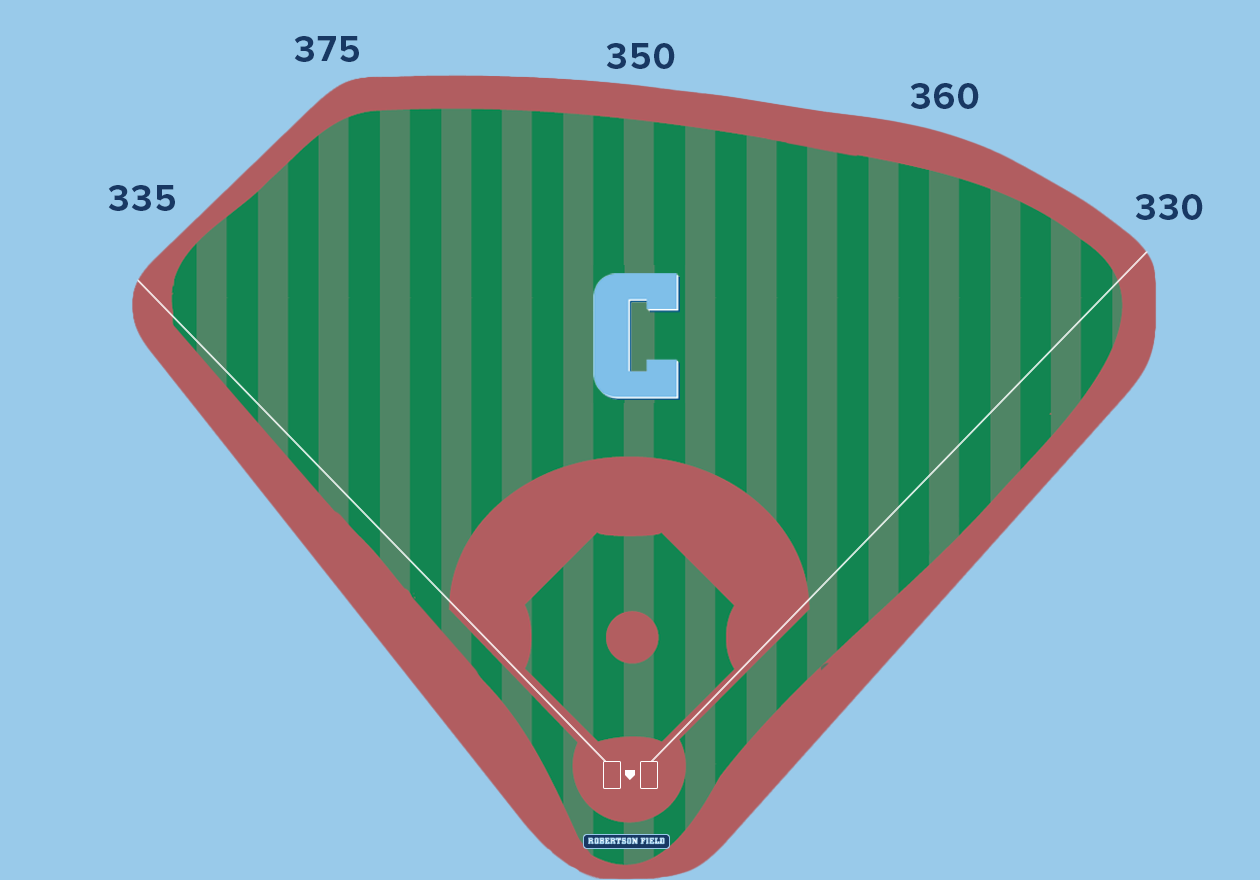
\includegraphics[height=8cm]{images/columbia_field.png}
    \caption{Robertson Field at Satow Stadium}
\end{figure}
\vspace{1cm}

Columbia's Robertson Field at Satow Stadium is known to be a hitter friendly ballpark, as it has a shallow outfield with relatively low fences. This means that in comparison to a standard ballpark, hitters are more likely to get home runs. It also has a relatively small foul territory leading to many foul balls landing on the nearby track or parking lot making them unable to be caught for a foul out.  \cite{columbialions2022baseball} \cite{columbialions2023baseball} \cite{columbialions2024baseball}

\newpage
\begin{figure}[h]
    \centering
    \begin{tabular}{c c c}  
        & \textbf{All NCAA Ballparks} & \textbf{Robertson Field} \\
        \multirow{2}{*}{\textbf{RHB}} &  
        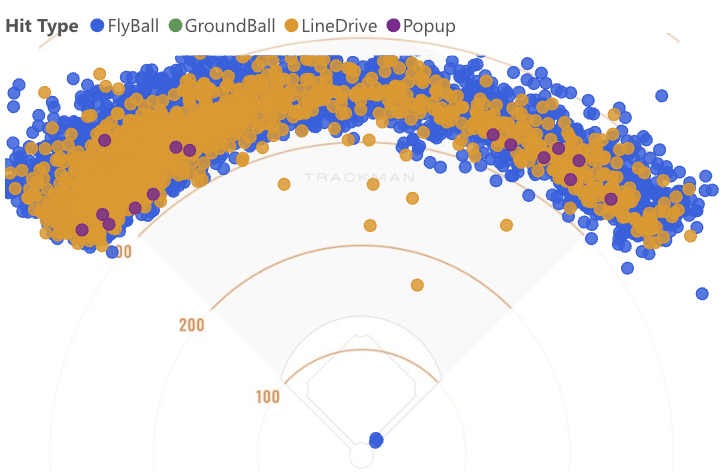
\includegraphics[width=0.45\textwidth]{images/RHB_homers24_NCAA.png} &  
        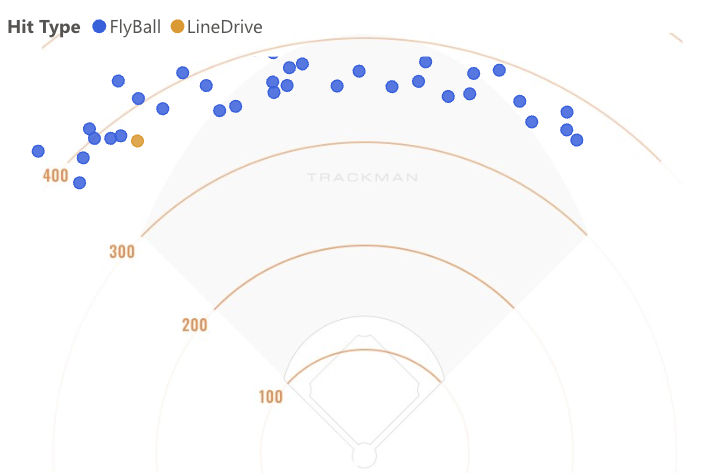
\includegraphics[width=0.45\textwidth]{images/RHB_homers24_Robertson.png} \\
        \multirow{2}{*}{\textbf{LHB}} &  
        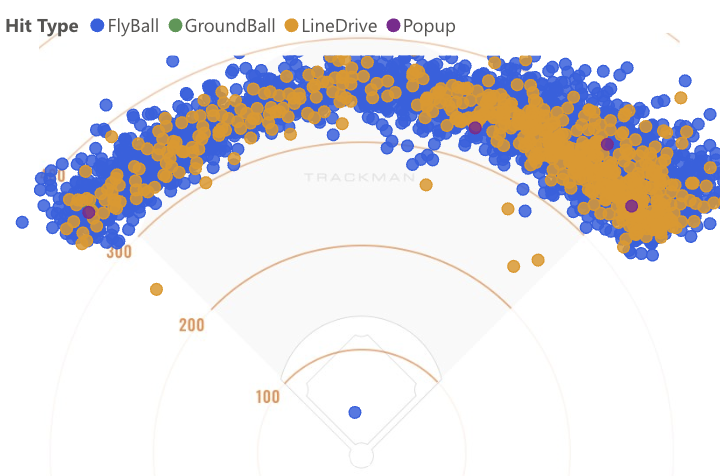
\includegraphics[width=0.45\textwidth]{images/LHB_homers24_NCAA.png} &  
        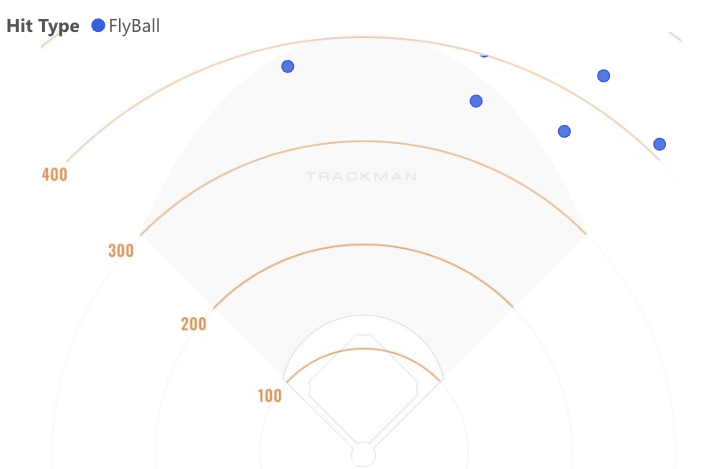
\includegraphics[width=0.45\textwidth]{images/LHB_homers24_Robertson.png} \\
    \end{tabular}
    \caption{Home Run Comparison 2024 – Robertson Field vs. All NCAA}
    \label{fig:heatmaps}
    \cite{trackman2024}
\end{figure}
\vspace{1cm}

Comparing home runs at Robertson Field to home runs across the NCAA DI allows us to see some of unique quirks of Robertson Field and the effect of handedness. Majority of home runs have been pulled by hitters resulting in left-handed batters hitting to deep right field and right-handed hitters to deep left. Across the NCAA and even with some right-handed hitters at Robertson Field there are some opposite field home runs but significantly less. 

Almost all of the home runs at Robertson Field are within the 400-foot barrier. This is partly due to Robertson Field's shallow outfield, which causes hits to leave the park that would otherwise stay in at other fields. This affects the ideal positioning of the outfield when playing at Robertson Field.

Each park's unique quirks and dimensions lead to adjustments in fielder positioning, particularly with the outfield. Due to this and Robertson Field's shallow outfield dimensions, my data was restricted to only games that Columbia played at home at Robertson Field.
\vspace{1cm}

\subsubsection{What is TrackMan and What it Measures}
TrackMan is a leading sports technology company that gathers relatively accurate ball and player tracking data for baseball and several other sports. TrackMan can produce reports on player data including things such as spray charts, heat maps, and zone breakdowns. It is used across many levels of baseball, including all thirty Major League Baseball teams, their minor league teams, most NCAA Division I baseball teams, and even premier summer leagues, such as the Cape Cod Baseball League. \cite{trackman2023baseball}


\subsubsection{Limitations in NCAA Data}
At the Major League Level, TrackMan is one of several ways that the league tracks player and ball data. The most used and accurate way that Major League Baseball tracks and quantifies almost all of the on field action is through a dozen Hawk-Eye cameras arrayed around each ballpark. These high-frame rate cameras are used to track and capture bat, pitch, player, and batted balls at an advanced level. The Hawk-Eye system has provided MLB with immense amounts of data for each action on the field. \cite{dawn2023hawkeye}

The NCAA is limited to TrackMan's technology for its player and ball tracking which is often installed differently in each ballpark and being manned by unpaid and inexperienced college students. Meaning that the NCAA is not only greatly limited in terms of data in comparison to MLB but that there are also often errors in NCAA TrackMan logs, especially with pitch type logging. 

Columbia's TrackMan files from the past three years do not include data on who the position players are. This means that I am unable to take into account who the individuals are in the defensive positions when evaluating the optimal locations for them. In an ideal world and at the Major League level, the defensive player is taken into account when evaluating their positioning placement, as player specific qualities and strength can effect their placement.  As a result of the specific player's not being logged in TrackMan, these player specific qualities - such as throwing hand, arm value, arm strength, range, and speed  - are all not included in this thesis. \cite{mlbsavant2023field} \cite{mlbsavant2023fielderpositioning}

Columbia's TrackMan data also does not capture any information of the environmental factors, such as weather and wind. Both of which can affect the movement of the ball and in turn the defensive positioning of players. \cite{mlb2023windimpact}

\newpage
\section{Data and Methodology}

\subsection{Data Collection}

As mentioned, I am primarily using Columbia University Baseball's TrackMan data from the $84$ home games played across the $2022$ \cite{trackman2022}, $2023$ \cite{trackman2023}, and $2024$ seasons \cite{trackman2024}. Each game Columbia has played during this time frame has two associated TrackMan files - the first contains information on the ball, the second has data on the position player's placement. Each game has a unique ID, as does each play and pitch that I grouped these data files on. 

The key variables from these data frames are: Game ID, Pitcher Arm, Batter Hand, Inning, Outs, Balls, Strikes, Pitch Call, K or BB, Tagged Hit Type, Play Result, Outs on Play, Detected Shift, and X and Z coordinates for each position player at the time of pitch release. 

These variables provide information on the current state of the game, the locations of each athlete of interest, and the result of the pitch. 

I also gathered more general information on NCAA Division I Baseball from TrackMan's Team Dashboards and Player Reports. \cite{trackman2022} \cite{trackman2023} \cite{trackman2024} \cite{trackman2023baseball}


\subsection{Exploring the Data (EDA)}

\subsubsection{Columbia Positioning}

The defensive positioning data consists of the X and Z coordinates for each position player at the time of pitch release. To better understand the positioning strategies Columbia uses, we can visualize the spatial distribution of players across different games using heatmaps. These heatmaps provide insight into typical defensive alignments and the frequency of certain positioning strategies.

\vspace{1cm}
\begin{figure}[h]
    \centering        
    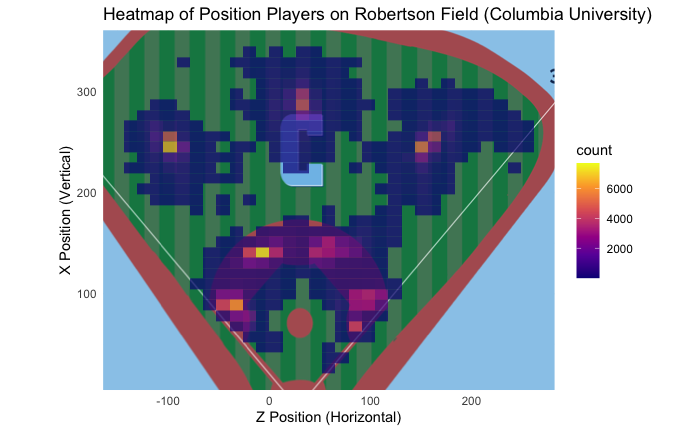
\includegraphics[height=10cm]{images/player_heatmap.png}
    \caption{Heatmap of Columbia Position Players at Pitch Release at Home - $2022$, $2023$, $2024$}
    \cite{trackman2022} \cite{trackman2023} \cite{trackman2024} \cite{albert2023analyzing}
\end{figure}
\vspace{1cm}

\newpage

This heatmap shows the locations of Columbia positions players during pitch release across the $2022$, $2023$, and $2024$ season when at home. There are three relatively distinct clusters in the outfield, aligning with the base positions for each of the three outfield positions. There is plenty of overlap in the infield, suggesting more defensive movement across the positions. 

\vspace{1cm}
\begin{figure}[h]
    \centering        
    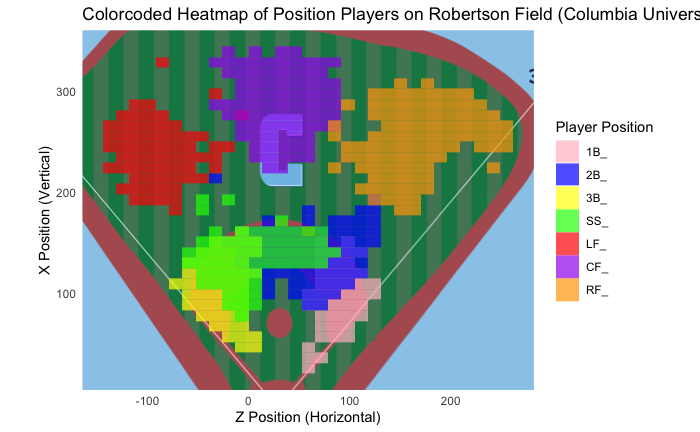
\includegraphics[height=10cm]{images/colorcoded_pos_heatmap.png}
    \caption{Color Coded Heatmap of Columbia Position Players at Pitch Release at Home - $2022$, $2023$, $2024$}
    \cite{trackman2022} \cite{trackman2023} \cite{trackman2024} \cite{albert2023analyzing}
\end{figure}
\vspace{1cm}
\newpage

Breaking down each position by color allows us to examine the unique area each position covers. The most significant overlap occurs in the middle infield, between second base and shortstop, which is expected, especially with the shift still being legal at the NCAA Division I level. There is also noticeable overlap between first and second base, as well as between third base and shortstop, indicating significant movement within the infield. The outfield positions are generally distinct, with small areas of overlap in center field. Additionally, there is some overlap between the infield and the shallow outfield, particularly with second base playing deeper and overlapping with right field.



\newpage

\begin{figure}[h]
    \centering
    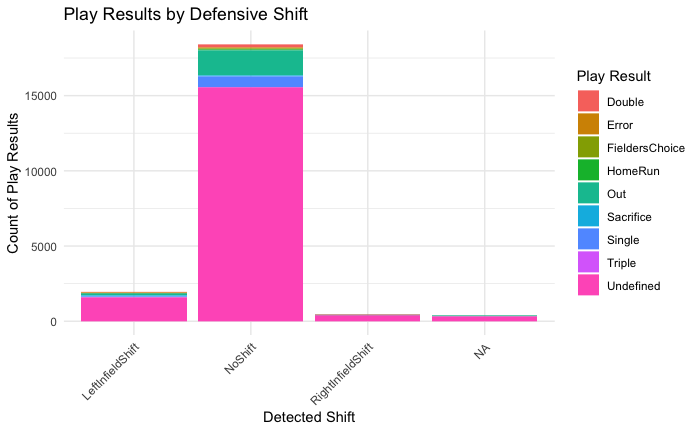
\includegraphics[height=10cm]{images/shift_breakdown.png}
    \caption{Play Result Across Shifting Techniques}
    \cite{trackman2022} \cite{trackman2023} \cite{trackman2024} \cite{albert2023analyzing}
\end{figure}
\vspace{1cm}

Furthermore, a detailed analysis of detected shifts shows the correlation between defensive shifts and play outcomes. Across the 2022, 2023, and 2024 seasons Columbia utilized a defensive shift during approximately $11.10\%$ of pitches thrown at home. When utilizing a defensive shift, the play result was an out approximately $8.932\%$ of the time. The play result was a hit (single, double, triple, home run) approximately $6.1\%$ of the time when the Columbia defense implemented a shift. 

\newpage
\begin{figure}[h]
    \centering
    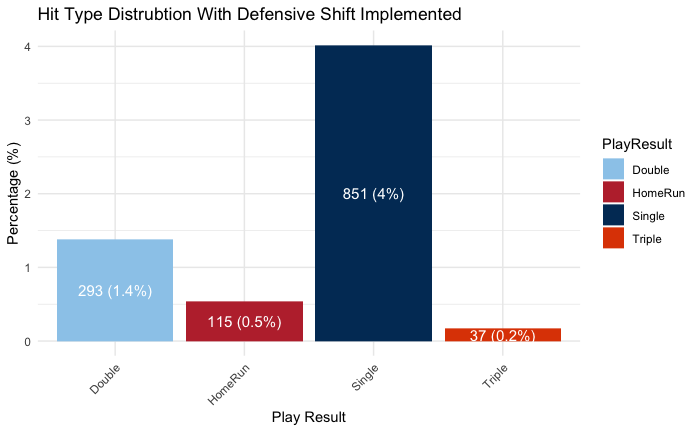
\includegraphics[height=10cm]{images/hits_against_shift.png}
    \caption{Hit Results Across Shifting Techniques}
    \cite{trackman2022} \cite{trackman2023} \cite{trackman2024} \cite{albert2023analyzing}
\end{figure}

Singles were the most common hit type when the shift was in effect, with $851$ singles allowed when shifting over the $2022$, $2023$, and $2024$ seasons. They were more common than all three of the other hit types combined when defensively shifting ($851$ v. $445$). 

As discussed in \ref{sec:platoon}, handedness plays a great role in what happens during an at bat. The handedness of both the pitcher and batter have a great effect on the likelihood of the result of an at bat and the location of the ball if contact is made. 

The following heatmaps breakdown the Columbia defensive positioning across each handedness match-up. 
It is worth noting how many more data points there are for right-handed pitchers than left-handed. 

\begin{figure}[h!]
    \centering
    \begin{minipage}{\textwidth}
        \centering
        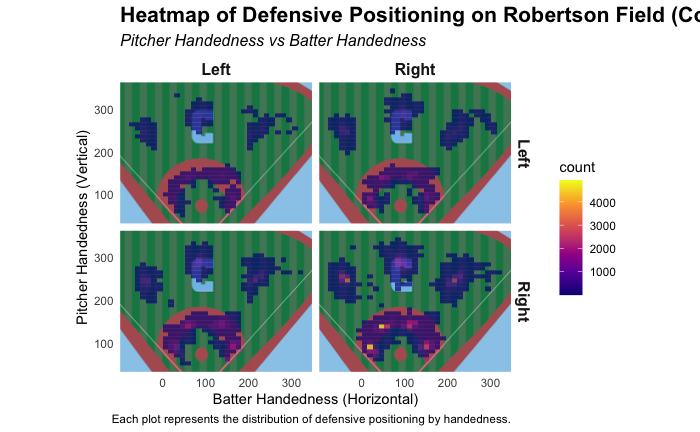
\includegraphics[height=10cm]{images/handedness_heatmap.png}
        \caption{Player Positioning During Different Handedness Match-Ups}
        \cite{trackman2022} \cite{trackman2023} \cite{trackman2024} \cite{albert2023analyzing}
    \end{minipage}

    \vspace{0.5cm} 

    \begin{minipage}{\textwidth}
        \centering
        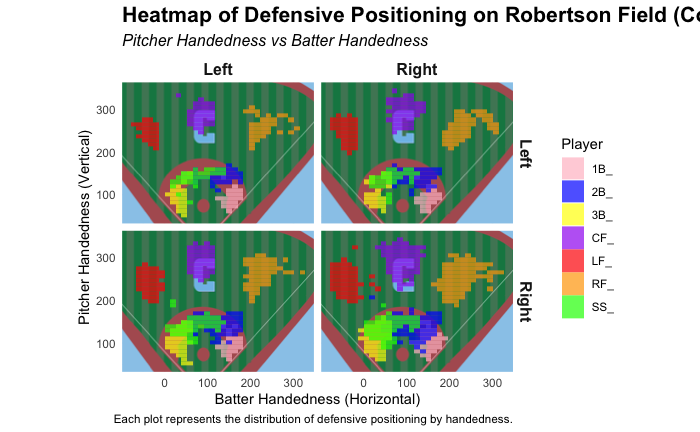
\includegraphics[height=10cm]{images/color_coded_handedness_heatmap.png}
        \caption{Color Coded Player Positioning During Different Handedness Match-Ups}
        \cite{trackman2022} \cite{trackman2023} \cite{trackman2024} \cite{albert2023analyzing}
    \end{minipage}
\end{figure}
\newpage


There are substantial differences in the amount of ground covered across the positions. To find the the total area covered by each position, I found the minimum and maximum X and Z values for each position and then computed the area of the bounding box using the following formula: 

$$Area = (max X-minX)*(maxZ-minZ)$$

The first baseman and third baseman cover the smallest areas on the field, with first base covering $6,118.4$ square units and third base covering $6,834.1$ square units. These positions are primarily responsible for their respective bases, limiting their coverage to the infield. This confined responsibility, with minimal range beyond the bases, results in significantly smaller coverage areas compared to other field positions. 

On the other hand, the second baseman and shortstop share coverage of second base and cover larger areas, which leads to higher total area coverage than the first and third basemen. The second baseman and shortstop also have more mobility within the infield, contributing to their larger areas. Within this data, the second baseman covers the largest area on the field, $19,464.1$ square units, almost $3,000$ more square units than any other position. 

\begin{figure}[h]
    \centering
    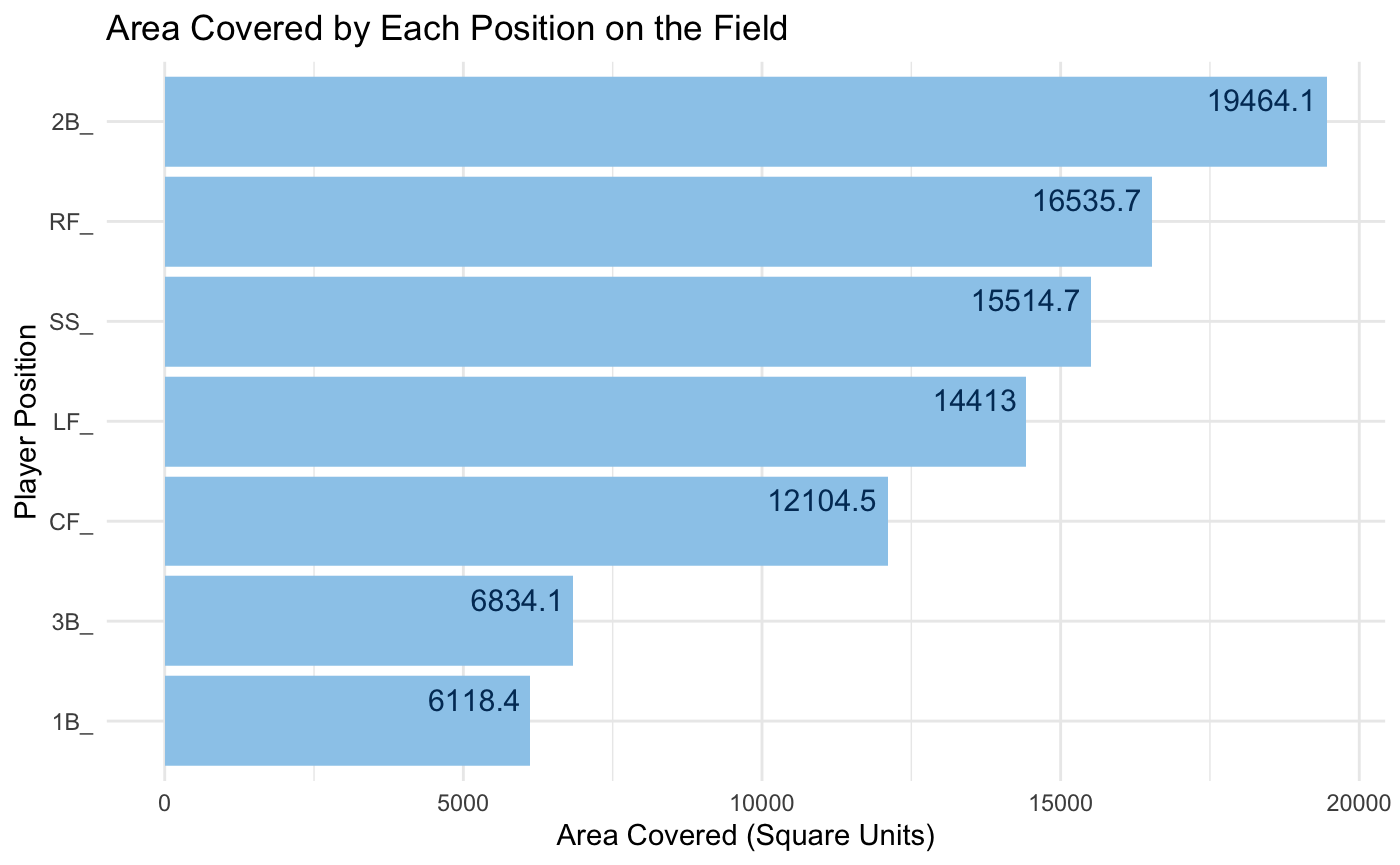
\includegraphics[height=10cm]{images/area_covered.png}
    \caption{Total Area Covered By Each Position At Robertson Field - 2022, 2023, 2024}
    \cite{trackman2022} \cite{trackman2023} \cite{trackman2024}
\end{figure}


\newpage
\subsubsection{Hitting at Robertson Field}

Each ballpark presents unique characteristics that can influence hitting patterns, Robertson Field is no exception. To explore this, we begin by analyzing batter performance based on their handedness and how it interacts with defensive positioning. We then visualize the hit locations and zones to see if any consistent patterns emerge for right- and left-handed batters.
\vspace{0.5cm} 
\begin{figure}[h]
    \centering
    \begin{tabular}{cc}  
        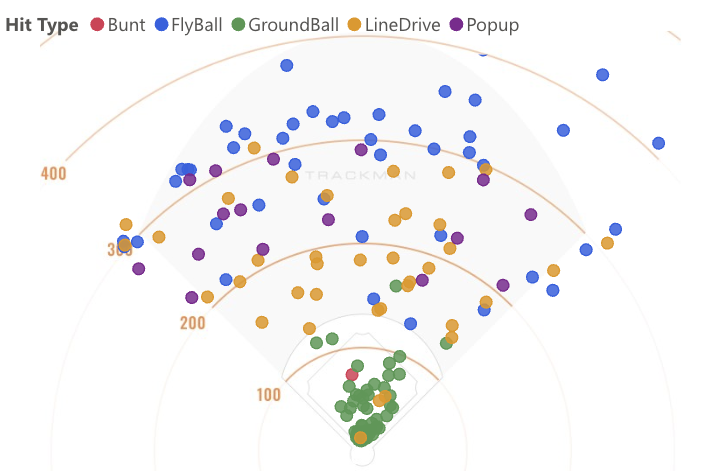
\includegraphics[width=0.5\textwidth]{images/LHB2024_spray_Robertson.png} & 
        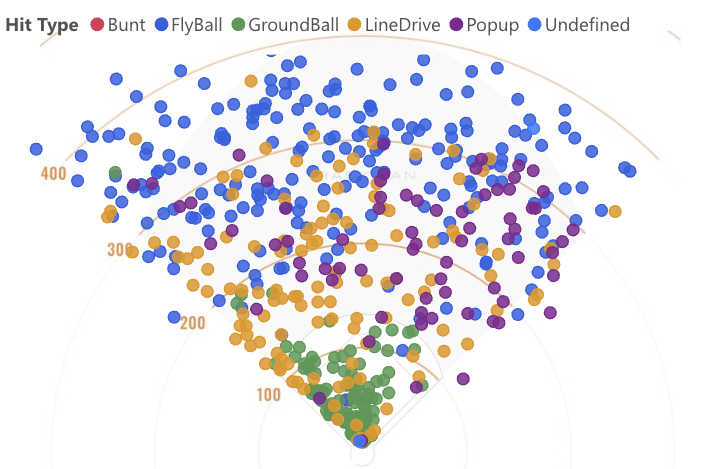
\includegraphics[width=0.5\textwidth]{images/RHB2024_spray_Robertson.png} \\
         Left-Handed Batter (LHB) & Right-Handed Batter (RHB)
    \end{tabular}
    \caption{Spray Charts for Left-Handed and Right-Handed Batters – 2024 Season at Robertson Field}
    \label{fig:spray_charts_batter_handedness}
    \cite{trackman2024} \cite{columbialions2024baseball}
\end{figure}
\vspace{.5cm}

The most obvious difference between the two spray charts is how many more hits there are from right-handed batters. As described earlier, we can also see that hitters tend to favor pulling the ball (right-handed batters hitting to left field and left-handed batters hitting to right field). 

To further explore the impact of handedness at Robertson Field, we will analyze batter zones, broken down by the batter's handedness and the opposing pitcher's throwing hand.

\newpage
\begin{figure}[h]
    \centering
    \begin{tabular}{c}  
        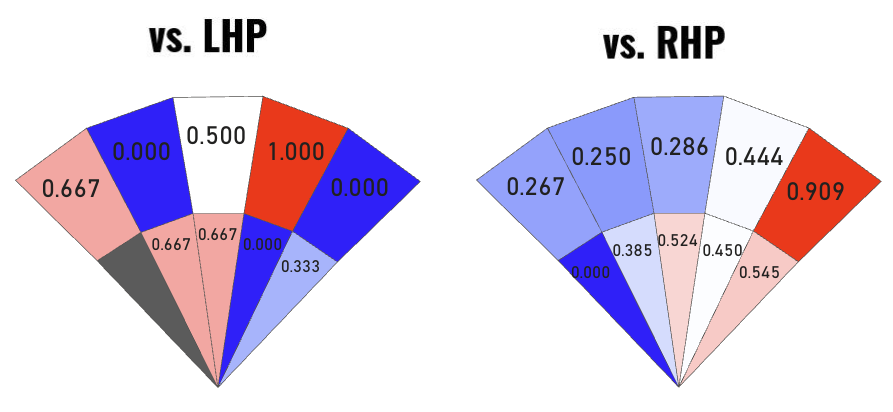
\includegraphics[width=0.8\textwidth]{images/LHB2024_zones_Robertson.png} \\
        \textbf{Left-Handed Batter (LHB) Zones} \\[1em]  
        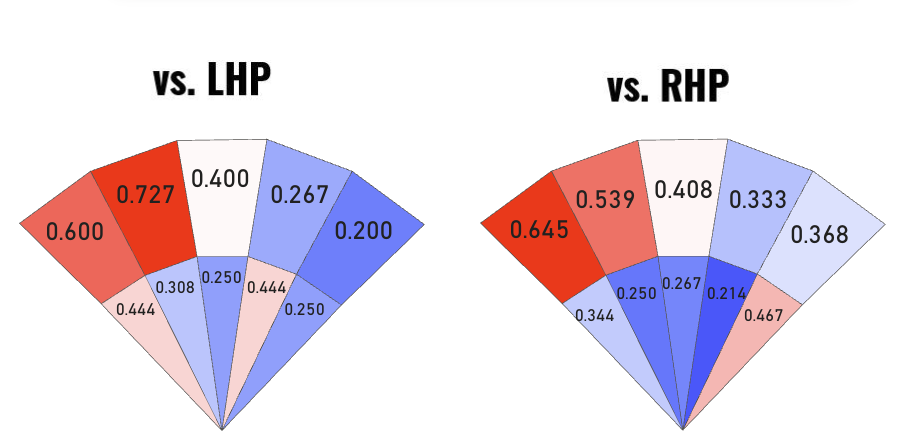
\includegraphics[width=0.8\textwidth]{images/RHB2024_zones__Robertson.png} \\
        \textbf{Right-Handed Batter (RHB) Zones} 
    \end{tabular}
    \caption{Zone distribution for batters at Robertson Field, split by handedness and pitcher’s hand.}
    \label{fig:batting_zones}
    \cite{trackman2024}
\end{figure}
\vspace{.7cm}

From these zones, we see the impact of a pitcher's hand on hit location, especially with left-handed batters. Lefty on lefty match-ups most often lead to hits landing in one of four zones, deep left field, center right field, or between second and third base on the infield. 

This differs from the lefty (batter) righty (pitcher) match-ups where batters are pulling the ball more as their hits are most often landing in deep right field, or between first and second. 

These differences are less drastic with right-handed batters, as the most frequent hit locations are still center to deep left field against both left- and right-handed pitchers. It is worth noticing that righty (batter) on righty (pitcher) match-ups lead to more balls being hit towards first base, while righty (batter) on lefty (pitcher) match-ups lead to hits either towards third base or between first and second. \cite{mlb2023left-handedpitching} \cite{appliedvision2023}

\newpage
\section{Models}

We will now dive into my models. The goal of these models is to to optimize defensive positioning for Columbia Baseball, focusing on batter and pitcher handedness to determine the best positions (X and Z) for each defensive position to maximize the probability of an "Out."

\subsection{Data Preparation}
\subsubsection{Feature Selection}
There are seventeen features that will be used across the models \cite{trackman2022} \cite{trackman2023} \cite{trackman2024}:

\begin{itemize}
    \item \textbf{PitchUID:} A unique identifier for each pitch. 
    \item \textbf{PitcherThrows:} The handedness of the pitcher, either left or right.
    \item \textbf{BatterSide:} The handedness of the batter, either left or right. Specific to the at bat, so switch hitters (players who can hit from both sides of the plate) are registered on an individual plate appearance.
    \item \textbf{PlayResult:} The result of the pitch. This has been changed to be binary, 1 = out, 0 = not out.
    \item \textbf{DetectedShift:} If an infield shift is detected on the current play. Three options: NoShift, there is no shift detected; LeftInfieldShift, the infield is shifted to the left of second base; or RightInfieldShift, the infield has shifted to the right of second base.
    \item \textbf{1B\_PositionAtReleaseX:} The vertical location on the field for the first baseman at the time of pitch release.
    \item \textbf{1B\_PositionAtReleaseZ:} The horizontal location on the field for the first baseman at the time of pitch release.
    \item \textbf{2B\_PositionAtReleaseX:} The vertical location on the field for the second baseman at the time of pitch release.
    \item \textbf{2B\_PositionAtReleaseZ:} The horizontal location on the field for the second baseman at the time of pitch release.
    \item \textbf{3B\_PositionAtReleaseX:} The vertical location on the field for the third baseman at the time of pitch release.
    \item \textbf{3B\_PositionAtReleaseZ:} The horizontal location on the field for the third baseman at the time of pitch release.
    \item \textbf{SS\_PositionAtReleaseX:} The vertical location on the field for the shortstop at the time of pitch release.
    \item \textbf{SS\_PositionAtReleaseZ:} The horizontal location on the field for the shortstop at the time of pitch release.
    \item \textbf{LF\_PositionAtReleaseX:} The vertical location on the field for the left fielder at the time of pitch release.
    \item \textbf{LF\_PositionAtReleaseZ:} The horizontal location on the field for the left fielder at the time of pitch release.
    \item \textbf{CF\_PositionAtReleaseX:} The vertical location on the field for the center fielder at the time of pitch release.
    \item \textbf{CF\_PositionAtReleaseZ:} The horizontal location on the field for the center fielder at the time of pitch release.
    \item \textbf{RF\_PositionAtReleaseX:} The vertical location on the field for the right fielder at the time of pitch release.
    \item \textbf{RF\_PositionAtReleaseZ:} The horizontal location on the field for the right fielder at the time of pitch release.
\end{itemize}

PlayResult will be the output variable to predict for my models. \textbf{The X and Z locations for each player, PitcherThrows, BatterSide, and DetectedShift are the features.} Categorical variables (BatterSide, PitcherThrows, DetectedShift) were converted to factors. 

There was originally $12,641$ pitches in this dataset. $10,684$ pitches had the result (PlayResult) "Undefined"; these were removed, leaving $1,957$ pitches to be examined. Of these $1,957$ pitches, $1,109$ of them resulted in an out, $56.67\%$. 

Below is a preview of the data, showing seven rows and the first seven columns. 

\begin{figure}[h]
    \centering
    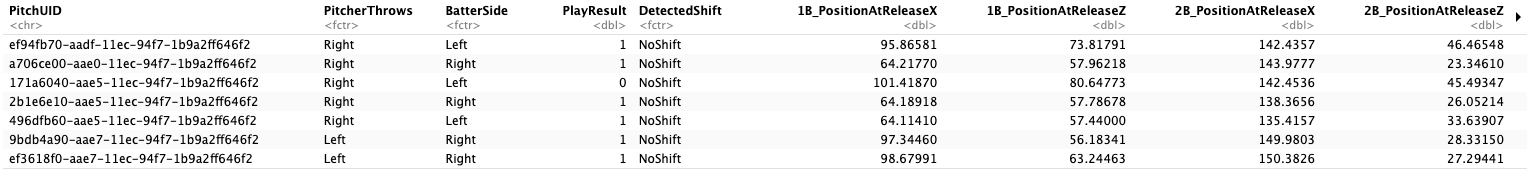
\includegraphics[height=3cm]{images/data_preview.png}
    \caption{Sample of Data}
    \cite{trackman2022}\cite{trackman2023}\cite{trackman2024}
\end{figure}

\subsubsection{Data Splitting}
For these models, the data was split into training and testing data; $80\%$ training, $20\%$ testing. A seed was set for reproducibility as the training and testing was randomly divided. 


\subsection{Logistic Regression Model}
\subsubsection{Model Introduction}
A logistic regression model was set up with the purpose of predicting PlayResult
based on BatterSide, PitcherThrows, DetectedShift, and the X and Z locations of each position player. The model was trained on the training data, tested on the testing data, and then evaluated using the following metrics: Receiver Operating Characteristic (ROC) Curve, Area Under the Curve (AUC), Confusion Matrix, and Accuracy. 

\subsubsection{Model Performance}
The model had $57.12\%$ accuracy, with the following results: 

\begin{table}[h!]
\centering
\begin{tabular}{|c|c|c|}
\hline
\multirow{2}{*}{Predicted} & \multicolumn{2}{c|}{Actual} \\ \cline{2-3} 
                           & 0   & 1   \\ \hline
0                          & 39  & 27  \\ \hline
1                          & 232 & 306 \\ \hline
\end{tabular}
\caption{Confusion Matrix - Logistic Regression}
\end{table}

This model seems to fail at picking up on the importance of batter and pitcher handedness, as the only significant predictors for the model are the following: 
\begin{itemize}
    \item \textbf{1B\_PositionAtReleaseZ:} P-Value = $0.0227$, the first baseman's z position affects the likelihood of an out
    \item \textbf{3B\_PositionAtReleaseX:} P-Value = $0.0155$, the X position of the third baseman plays a role in determining the outcome 
    \item \textbf{SS\_PositionAtReleaseZ:} P-Value = $0.00108$, indicating that the shortstop's Z position has a great influence on the play result 
    \item \textbf{DetectedShiftRightInfieldShift:} P-Value = $0.00193$, suggesting that when a right infield shift is used the likelihood of an out increases significantly 
\end{itemize}

\begin{figure}[h]
    \centering
    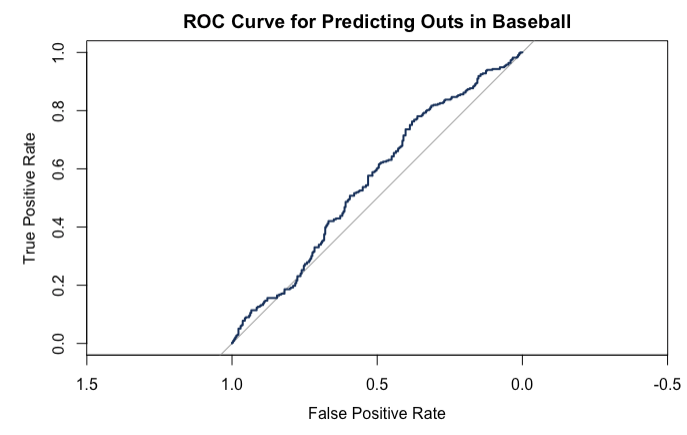
\includegraphics[height=10cm]{images/roc_lr.png}
    \caption{Receiver Operating Characteristic (ROC) curve showing logistic regression model's performance in predicting "out" plays (PlayResult = 1) based on player positioning, batter handedness, pitcher handedness, and detected shifts.}
\end{figure}

The AUC is $0.56$, slightly above the randomness threshold ($0.5$), suggesting that the model is not performing exceptionally well in distinguishing between out and non-out plays.

While the model is performing better than random guessing there is still significant room for improvement. 

\subsection{XGBoost Model}
\subsubsection{Model Introduction}
XGBoost (Extreme Gradient Boosting) is a highly efficient and accurate machine learning model, particularly well-suited for large datasets. It excels at handling missing data and uses parallel processing to speed up training. An XGBoost model was developed to predict the play result ($1$ = out, $0$ = not out) for each pitch, based on pitcher and batter handedness, defensive shift implementation, and the X and Z coordinates for each defensive player at the time of pitch release.

The model was trained on the training data and tested on the testing data. Cross-validation was then employed to determine the optimal number of boosting rounds ($100$), ensuring the model was tuned for maximum predictive performance and to avoid overfitting. It was subsequently evaluated using the following metrics: Receiver Operating Characteristic (ROC) Curve, Area Under the Curve (AUC), Confusion Matrix, and Accuracy.


\subsubsection{Model Performance}
The results from the XGBoost model demonstrate relatively strong performance in predicting the play result for each pitch, with an accuracy of $74.83\%$ and the following results. 

\begin{table}[h!]
\centering
\begin{tabular}{|c|c|c|}
\hline
\multirow{2}{*}{Predicted} & \multicolumn{2}{c|}{Actual} \\ \cline{2-3} 
                           & 0   & 1   \\ \hline
0                          & 170  & 51  \\ \hline
1                          & 101 & 282 \\ \hline
\end{tabular}
\caption{Confusion Matrix - XGBoost Model}
\end{table}
\newpage
\begin{figure}[h]
    \centering
    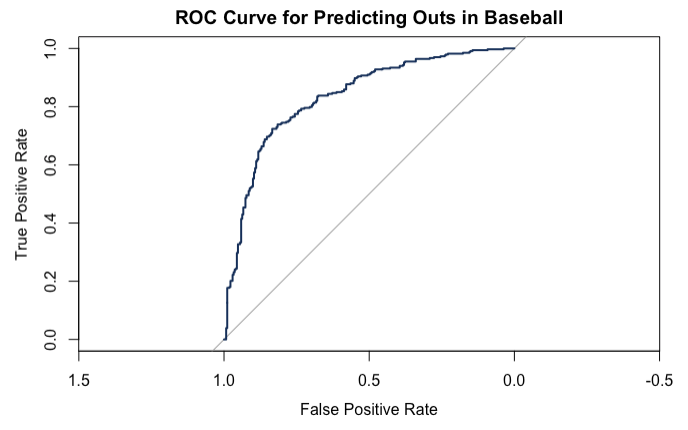
\includegraphics[height=10cm]{images/roc_xgb.png}
    \caption{Receiver Operating Characteristic (ROC) curve showing XGBoost model's performance in predicting "out" plays (PlayResult = 1) based on player positioning, batter handedness, pitcher handedness, and detected shifts.}
\end{figure}
\vspace{.5cm}

The AUC is $0.83$, significantly above the randomness threshold ($0.5$), suggesting that the model performs reasonably well in distinguishing between out and non-out pitches. While the model performs reasonably well, there is still room for improvement through further tuning or more complex models.


\subsection{Random Forest Model}
\subsubsection{Model Introduction}
Random Forest is an ensemble machine learning method often used for regression and classification with large datasets. It combines multiple decision trees to reduce overfitting and improve accuracy. A random forest model was developed to predict the play result ($1$ = out, $0$ = not out) for each pitch, based on pitcher and batter handedness, defensive shift implementation, and the X and Z coordinates for each defensive player at the time of pitch release.

The model was trained on the training data and tested on the testing data. Cross-validation was employed to tune the hyperparameters and determine the optimal number of variables per split (mtry), using a grid search with values $3$, $5$, and $7$. This ensured the model was optimized for predictive performance while minimizing overfitting. The model was evaluated using the following metrics: Receiver Operating Characteristic (ROC) Curve, Area Under the Curve (AUC), Confusion Matrix, and Accuracy. 

\subsubsection{Model Performance}

The results from the Random Forest model demonstrate a relatively strong performance in predicting the play result for each pitch, with an accuracy of $75.50\%$ and the following results. 

\begin{table}[h!]
\centering
\begin{tabular}{|c|c|c|}
\hline
\multirow{2}{*}{Predicted} & \multicolumn{2}{c|}{Actual} \\ \cline{2-3} 
                           & 0   & 1   \\ \hline
0                          & 164  & 41  \\ \hline
1                          & 107 & 292 \\ \hline
\end{tabular}
\caption{Confusion Matrix - Random Forest Model}
\end{table}
\vspace{.4cm}
\begin{figure}[h]
    \centering
    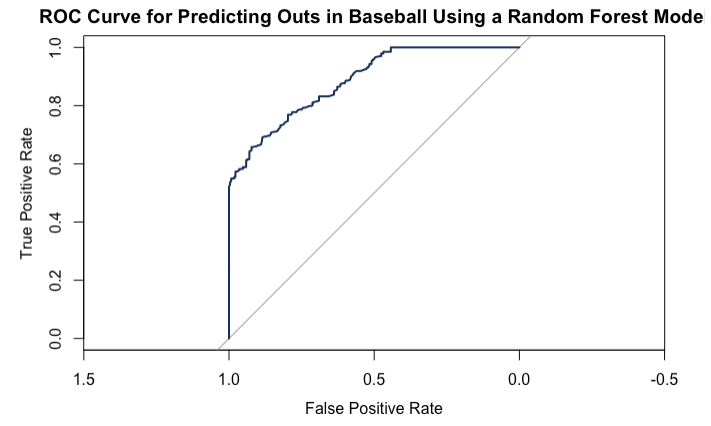
\includegraphics[height=10cm]{images/roc_rf.png}
    \caption{Receiver Operating Characteristic (ROC) curve showing Random Forest model's performance in predicting "out" plays (PlayResult = 1) based on player positioning, batter handedness, pitcher handedness, and detected shifts.}
\end{figure}
\vspace{.7cm}

The AUC is $0.56$, marginally above the randomness threshold ($0.5$), suggesting that the model performs slightly better than random guessing in distinguishing between out and non-out pitches. While the accuracy indicates a relatively strong performance from the model the AUC suggests that there is significant room for improvement.

\subsection{Comparing Models}
There were various results across the three models: 

\begin{table}[h!]
\centering
\begin{tabular}{|c|c|c|c|}
\hline
& \textbf{Logistic Regression}  & \textbf{XGBoost} & \textbf{Random Forest} \\
\hline
\textit{Accuracy} & $57.12\%$ & $74.83\%$ & $75.50\%$\\
\textit{Precision} & $56.88\%$ & $73.63\%$ & $73.18\%$\\
\textit{Recall} & $91.89\%$ & $84.68\%$ & $87.69\%$\\
\textit{AUC} &  $0.56$  & $.83$ & $0.56$ \\
\hline
\end{tabular}
\caption{Comparing the Models}
\end{table}


\vspace{.4cm}
\begin{figure}[h]
    \centering
    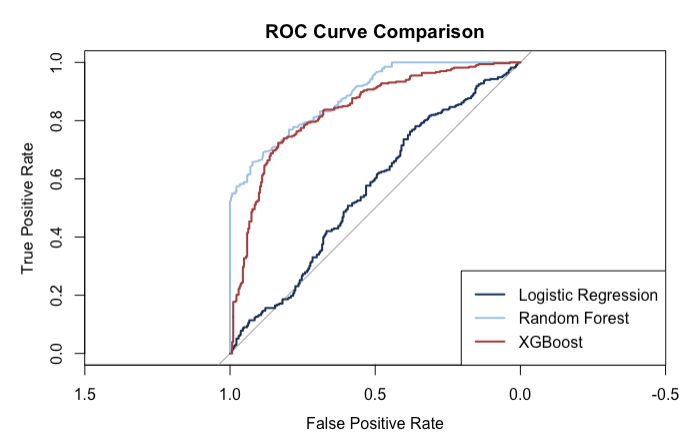
\includegraphics[height=10cm]{images/roc_comp.png}
    \caption{Receiver Operating Characteristic (ROC) curve showing Logistic Regression, XGBoost, and Random Forest models' performances in predicting "out" plays (PlayResult = 1) based on player positioning, batter handedness, pitcher handedness, and detected shifts.}
\end{figure}
\vspace{.7cm}

Among the models, the XGBoost and Random Forest models showed similar performance in terms of accuracy, precision, and recall, with the XGBoost model performing slightly better in terms of AUC ($0.83$). The Logistic Regression model, while providing the best precision ($56.88\%$) and recall ($91.89\%$), suffered from low accuracy ($57\%$) and AUC ($0.56$), which is barely above the randomness threshold ($0.5$).

These results indicate that XGBoost and Random Forest are more effective at fitting the data and providing accurate predictions. The XGBoost model, in particular, stands out due to its significantly higher AUC, making it the best-performing model among the three. Given this, I chose to focus on improving the XGBoost model for further optimization.

\subsection{Optimization Strategy}
\subsubsection{Improving the XGBoost Model}
To better my XGBoost model, I first added a new feature, \textit{BatterPitcherIntercation}, to capture the relationship between the handedness of the batter and the pitcher. 

I then performed a grid search to tune the hyperparameters effectively to optimize the model. The grid search found that $46$ rounds was ideal for the parameters. 

This updated model was a slight improvement from the previous models. The results indicated a relatively strong performance in predicting the play result for each pitch, with an accuracy of $75.50\%$ and the following results. 

\begin{table}[h!]
\centering
\begin{tabular}{|c|c|c|}
\hline
\multirow{2}{*}{Predicted} & \multicolumn{2}{c|}{Actual} \\ \cline{2-3} 
                           & 0   & 1   \\ \hline
0                          & 135  & 35  \\ \hline
1                          & 136 & 298 \\ \hline
\end{tabular}
\caption{Confusion Matrix - Random Forest Model}
\end{table}


\textbf{Precision: } $68.66\%$ 


\textbf{Recall: } $89.49\%$

\vspace{.4cm}
\begin{figure}[h]
    \centering
    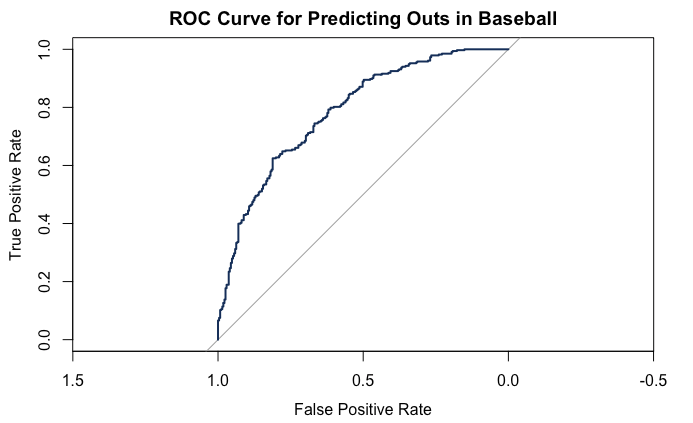
\includegraphics[height=10cm]{images/roc_final.png}
    \caption{Receiver Operating Characteristic (ROC) curve showing updated XGBoost model's performance in predicting "out" plays (PlayResult = 1) based on player positioning, batter handedness, pitcher handedness, and detected shifts.}
\end{figure}
\vspace{.7cm}

The AUC is $0.79$, significantly above the randomness threshold ($0.5$), suggesting that the model performs substantially better than random guessing in distinguishing between out and non-out pitches. 

\subsubsection{Optimal Positions}
Using the updated XGBoost model results, I calculated the predicted probabilities for each player's position and then grouped the data based on BatterPitcherInteraction and player position (X, Z) to identify the optimal position for each player in each handedness match-up. The results are summarized in the table below. Each table entry corresponds to the ideal coordinates (X, Z) for a given player, depending on whether the batter is left-handed or right-handed and whether the pitcher is left-handed or right-handed.

\vspace{.7cm}
\begin{table}[h!]
\centering
% Adjusting row height
\renewcommand{\arraystretch}{1.7}  
\resizebox{\textwidth}{!}{ 
\begin{tabular}{|c|c|c|c|c|}
\hline
 & \textbf{LvL}  & \textbf{LvR} & \textbf{RvR}  & \textbf{RvL} \\
\hline
\textit{First Baseman:} & $(89.41, 75.16)$ & $(88.02, 69.76)$ & $(98.16, 43.50)$ &  $(92.06, 61.82)$\\ \hline
\textit{Second Baseman:} & $(139.93, 60.60)$& $(154.73, 40.93)$ & $(148.02, -25.21)$ &  $(147.02, 40.17)$\\ \hline
\textit{Third Baseman:} & $(87.01, -55.60)$& $(77.72, -53.58)$ & $(95.17, -75.47)$ &  $(89.18, -67.64)$\\ \hline
\textit{Shortstop:} &  $(138.87, 10.64)$ & $(138.48, -32.01)$ & $(131.52, -59.02)$ &  $(138.78, -43.64)$\\ \hline
\textit{Left Fielder:} &  $(253.75, -106.45)$ & $(231.08, -112.52)$ & $(245.75, -136.4)$ &  $(249.96, -134.48)$\\ \hline
\textit{Center Fielder:} & $(287.12, 21.31)$ & $(285.51, -15.81)$ & $(315.0, -31.31)$ &  $(268.96, 14.97)$\\ \hline
\textit{Right Fielder:} & $(238.70, 135.58)$ & $(255.24, 133.69)$ & $(275.88, 106.1)$ &  $(225.21, 119.22)$\\ \hline
\end{tabular}
}
\caption{Optimal Positions}
\caption*{LvL = Left-handed batter vs. Left-handed pitcher, LvR = Left-handed batter vs. Right-handed pitcher, RvR = Right-handed batter vs. Right-handed pitcher, RvL = Right-handed batter vs. Left-handed pitcher.}
\end{table}
\vspace{.5cm}

\newpage
\begin{figure}[h]
    \centering
    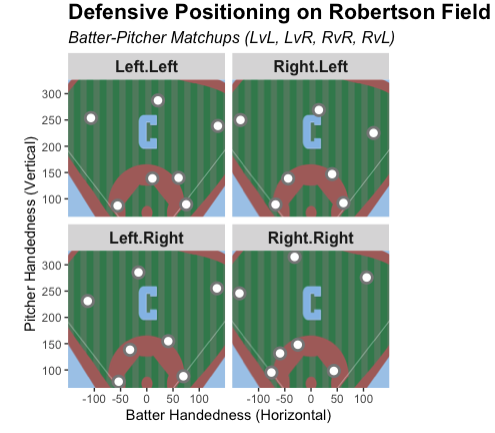
\includegraphics[height=13cm]{images/optimal_pos.png}
    \caption{Each plot represents the ideal defensive positions for each player based on the batter-pitcher hand match-up}
    \cite{trackman2022}\cite{trackman2022}\cite{trackman2024}
\end{figure}

The plots above show the ideal defensive positions for each player based on the batter-pitcher handedness match-up. Each dot represents the calculated optimal position for a player at a given BatterPitcherInteraction. The images are overlaid on a diagram of Columbia's field, with (X, Z) coordinates indicating the ideal position based on the model’s prediction.

There are noticeable differences in the positioning of the defensive players across the four plots, especially with the infielders. The second baseman and shortstop seem to move the most depending on the match-up. Infield shifts are noticeable for both same-hand match-ups — right infield shift (first baseman, second baseman, shortstop all to the right of second base) for the lefty-on-lefty match-up, and left infield shift (first baseman, second baseman, shortstop all to the left of second base) for the righty-on-righty match-up.

The outfield, first baseman, and third baseman remain more consistent with their placement across the different match-ups. These trends are useful for understanding the model's ability to predict optimal defensive positions based on batter-pitcher handedness match-ups.


\newpage
\begin{figure}[h]
    \centering
    \begin{tabular}{cc}  
        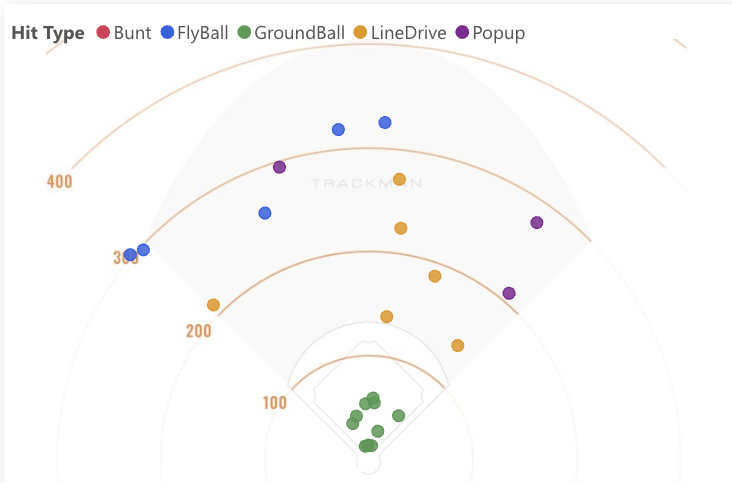
\includegraphics[width=0.5\textwidth]{images/spray24_lvl.png} & 
        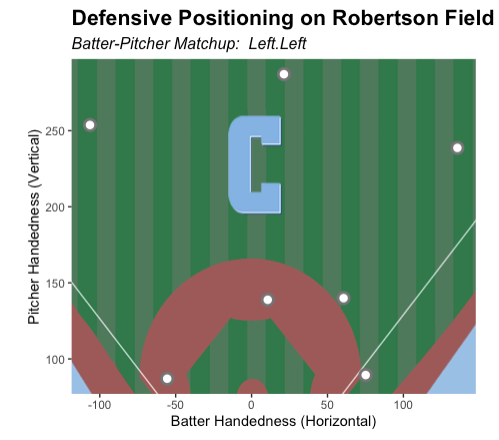
\includegraphics[width=0.5\textwidth]{images/optimal_lvl.png} \\
         LvL Spray Chart at Robertson Field - 2024 & Optimal Defensive Positioning for LvL
    \end{tabular}
    \caption{Lefty (Batter) v Lefty (Pitcher)}
    \label{fig:leftyvleftycomp}
    \cite{trackman2024}
\end{figure}
\vspace{.5cm}
\begin{figure}[h]
    \centering
    \begin{tabular}{cc}  
        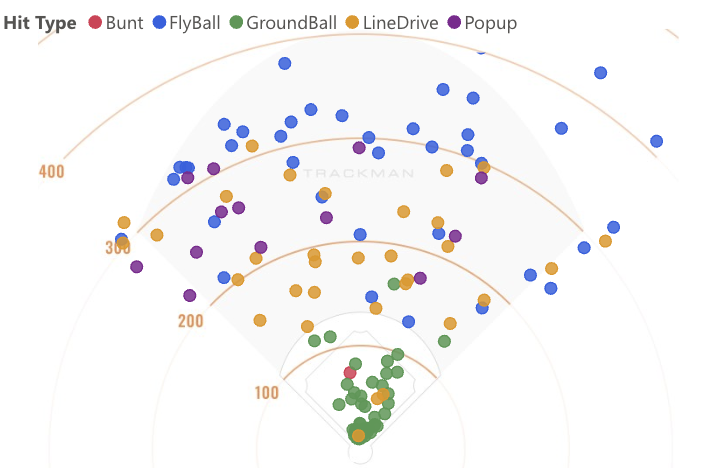
\includegraphics[width=0.5\textwidth]{images/spray24_lvr.png} & 
        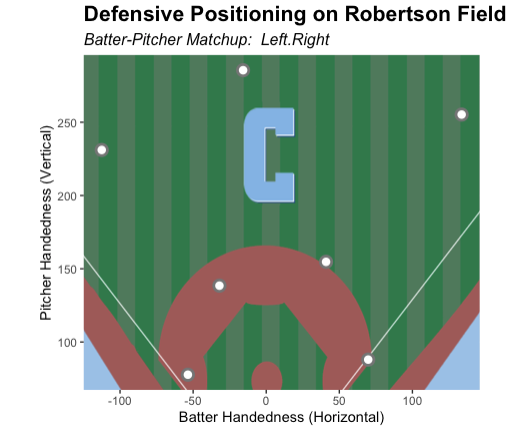
\includegraphics[width=0.5\textwidth]{images/optimal_lvr.png} \\
         LvR Spray Chart at Robertson Field - 2024 & Optimal Defensive Positioning for LvR
    \end{tabular}
    \caption{Lefty (Batter) v Righty (Pitcher)}
    \label{fig:leftyvrightycomp}
    \cite{trackman2024}
\end{figure}
\newpage
\begin{figure}[h]
    \centering
    \begin{tabular}{cc}  
        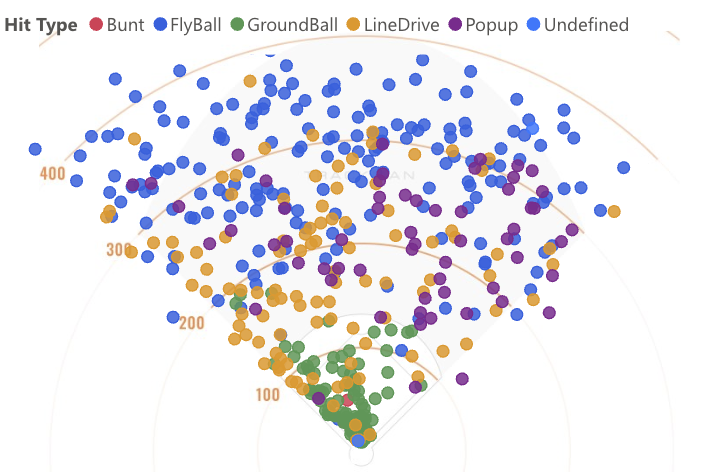
\includegraphics[width=0.5\textwidth]{images/spray24_rvr.png} & 
        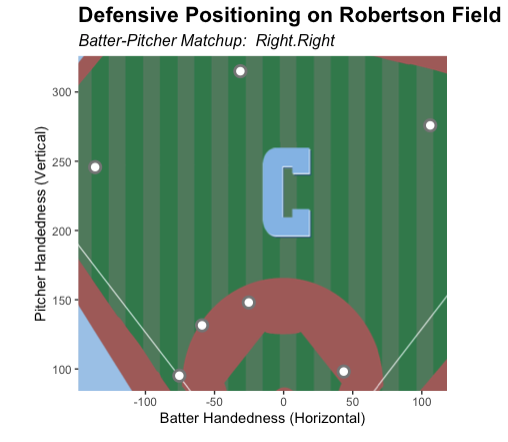
\includegraphics[width=0.5\textwidth]{images/optimal_rvr.png} \\
         RvR Spray Chart at Robertson Field - 2024 & Optimal Defensive Positioning for RvR
    \end{tabular}
    \caption{Righty (Batter) v Righty (Pitcher)}
    \label{fig:rightyvrightycomp}
    \cite{trackman2024}
\end{figure}
\vspace{.5cm}
\begin{figure}[h]
    \centering
    \begin{tabular}{cc}  
        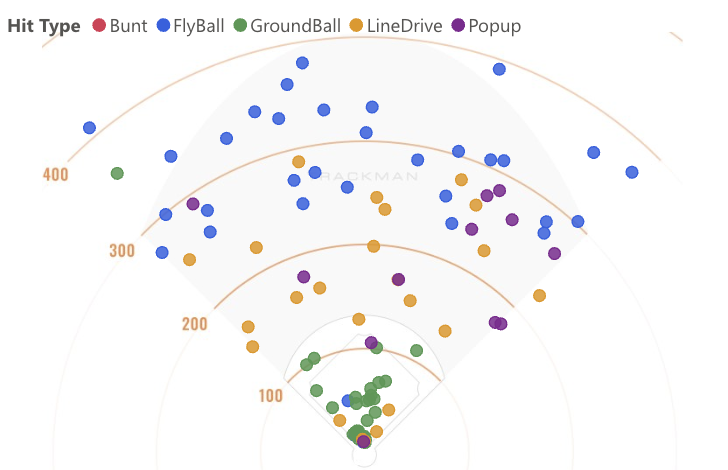
\includegraphics[width=0.5\textwidth]{images/spray24_rvl.png} & 
        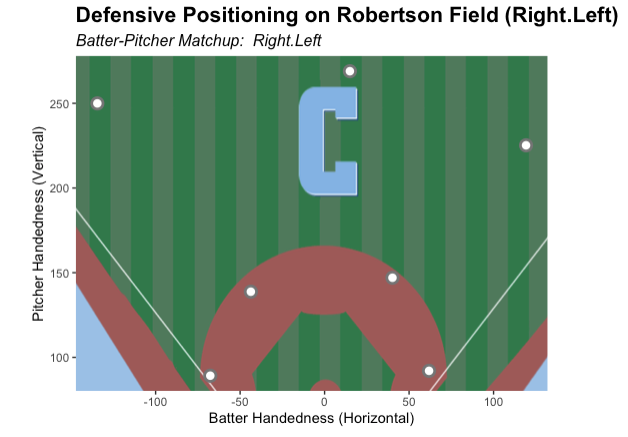
\includegraphics[width=0.5\textwidth]{images/optimal_rvl.png} \\
         RvL Spray Chart at Robertson Field - 2024 & Optimal Defensive Positioning for RvL
    \end{tabular}
    \caption{Righty (Batter) v Lefty (Pitcher)}
    \label{fig:rightyvleftycomp}
    \cite{trackman2024}
\end{figure}
\vspace{.5cm}

The plots above show the spray charts at Robertson Field in 2024 for each handedness match-up next to the optimal positions for each player for the same match-up. There are areas of the field favored for each match-up, and the model predicts the optimal positions accordingly. The model has been quite accurate, as it seems to be predicting the optimal positions for each player based on the most favored hitting locations for each batter-pitcher match-up.  

\newpage
\section{Conclusions and Future Directions}

The aim of this project was to develop a predictive model to optimize defensive positions in NCAA baseball, specifically for Columbia University, with the goal of maximizing outs based on batter-pitcher handedness and other relevant features. By leveraging TrackMan data and employing an XGBoost model, this thesis provides insights into how defensive positioning can be fine-tuned to improve performance.

The model demonstrated a high level of accuracy (75.50\%) in predicting the optimal positioning for each player. Notably, it identified significant shifts in the positioning of middle infielders based on batter-pitcher handedness match-ups. These findings highlight the importance of dynamic defensive strategies in baseball, emphasizing that defensive positioning should adapt to the batter's tendencies and the pitcher's characteristics.

This model could be implemented by Columbia Baseball in real games to inform coaching strategies and assist players in adjusting to various batting tendencies. By optimizing fielding positions, the team can increase the likelihood of converting balls in play into outs, providing a competitive advantage during games.


\subsection{Future Directions}
While this model has shown promise, there are several opportunities to improve its performance and adapt it to real-world applications:

\begin{itemize}
    \item \textbf{Continuously Update the Model's Data:} 
    The models used TrackMan data from Columbia Baseball's 2022, 2023, and 2024 \cite{trackman2022}\cite{trackman2022}\cite{trackman2024} seasons. Future updates after each game in 2025 (and beyond) could incorporate new data, further enhancing model accuracy and making it more adaptable to changes in player performance and batting trends.
    
    \item \textbf{Incorporating New Features:} 
    
    Although TrackMan data offers valuable insights, the model could be improved by incorporating additional features not included in the data files. Some of these features may be more relevant to higher levels of baseball, but others, such as player identification and weather, are accessible and could make the model more tailored to individual players and games.

    
    \item \textbf{Weather Data:} 
    Bringing in weather features to update the model for a specific game could also improve the likelihood of an out. Weather has a great affect on the movement of the ball, and bringing in weather patterns such as wind velocity, wind direction, humidity, and temperature would provide more information on how the ball is traveling that day. \cite{mlb2023windimpact}

    
    \item \textbf{Access to Raw Hit Data:} 
    The greatest enhancement to this model would come from access to raw ball hit location data. While some data was semi-accessible via the TrackMan Portal, the model’s predictions could be made more accurate if detailed information on hit locations was available. This would allow for precise positioning of players based on the actual trajectory of the ball, rather than relying on general tendencies.\cite{mlbsavant2023fielderpositioning} \cite{mlbsavant2023field} \cite{mlbsavant2023catchprobability} 
\end{itemize}

 
 The model could also be adapted for use by other NCAA teams. By inputting their team's data, other teams could implement similar strategies to optimize defensive positioning based on their specific players' tendencies. This could help bring data-driven decision-making to a broader range of teams, increasing the model's impact across college baseball.

\subsection{Final Thoughts}
The model developed in this project provides a data-driven approach to optimizing defensive positioning, with a focus on maximizing outs based on batter-pitcher handedness match-ups. By continually refining the model with more data and features, and by integrating real-time factors like weather, Columbia Baseball and other NCAA Division I teams can gain a significant advantage on the field. Major League Baseball teams already utilize similar, more advanced models to limit hits and maximize outs. As baseball becomes increasingly data-driven, teams have the opportunity to leverage their data through adaptive models like this one, enabling them to dynamically optimize performance and gain a competitive edge.


\newpage
\printbibliography

\section*{Supplementary Files}
You can find the code for this project in my GitHub repository:

\begin{itemize}
    \item \href{https://github.com/lillianmbradley/Undergraduate-Thesis}{GitHub Repository}
\end{itemize}
 

\end{document}